%% Parts of the formatting were taken from a template with the following
%% information:
%%
%% This template was created by PhD student Chris Zeoli in spring 2011 to meet
%% the University of Idaho College of Graduate Studies requirements for a PhD
%% Thesis.
%%
%% Updated by Graduate Student Juan Marulanda in Fall 2013 under the supervision
%% of Thesis and Dissertation Formatting Advisor Melinda Deyasi from the College
%% of Graduate Studies at University of Idaho
%% Contact: maru2593@vandals.uidaho.edu

\documentclass[12pt,letterpaper]{report}
\usepackage{float}
\usepackage{amssymb}
\usepackage{amsmath}
\usepackage{url}
\usepackage{accents}
\usepackage{bm}
\usepackage{tocloft}
\usepackage{amsfonts}
\usepackage{indentfirst}
\usepackage{tabto}

\renewcommand{\cftpartleader}{\cftdotfill{\cftdotsep}} % for parts
\renewcommand{\cftchapleader}{\cftdotfill{\cftdotsep}} % for chapters
\renewcommand{\cftsecleader}{\cftdotfill{\cftdotsep}} % for sections

%Allows placement of graphics.
%Recommended packages for figures and subfigures that fits this templates
\usepackage[pdftex]{graphicx}
\usepackage{caption}
\usepackage{subcaption}
%Allows fcns like doublespace, singlespace, and singlehalfspacing of text.
\usepackage{setspace}

\newcommand{\ubar}[1]{\underaccent{\bar}#1}
\DeclareMathOperator*{\argmin}{arg\,min}
\DeclareMathOperator*{\Geom}{\operatorname{Geom}}
\DeclareMathOperator*{\Read}{\operatorname{Read}}

\title{\textbf{MMC: THE DEVELOPMENT OF THE MIXTURE MODEL CACHING ALGORITHM}}
%Clears plain-page pg# settings, relocates pg#'s @ top-right-corner.
\makeatletter
\renewcommand*\l@section{\@dottedtocline{1}{1.5em}{2.3em}}
\renewcommand{\ps@plain}{
\renewcommand\@oddhead{\hfill\normalfont\textrm{\thepage}}
\renewcommand\@evenhead{}
\renewcommand\@oddfoot{}
\renewcommand\@evenfoot{}}
\renewcommand{\arraystretch}{1.5}

%Reduces space between section headings and top margin
\def\@makechapterhead#1{%
  \vspace*{-40\p@}%
  {\parindent \z@ \raggedright \normalfont
    \ifnum \c@secnumdepth >\m@ne
        \center\large\bfseries \@chapapp\space \thechapter : \space  #1\par\nobreak
        %\center\large\bfseries \thechapter : #1\par\nobreak
        \par\nobreak
        \vskip 10\p@
  }}

\def\@makeschapterhead#1{%
  \vspace*{-40\p@}%
  {\parindent \z@ \raggedright
    \normalfont
    \interlinepenalty\@M
    \center\large \bfseries  #1\par\nobreak
    \vskip 10\p@
  }}

\renewcommand\section{\@startsection{section}{1}{\z@}%
                                  {-3.5ex \@plus -1ex \@minus -.2ex}%
                                  {2.3ex \@plus.2ex}%
                                  {\normalfont\large\bfseries}}

\renewcommand\subsection{\@startsection{subsection}{1}{\z@}%
                                  {-3.5ex \@plus -1ex \@minus -.2ex}%
                                  {2.3ex \@plus.2ex}%
                                  {\normalfont\large\bfseries}}

\makeatother

%Changes leading pg#'s to roman sytle
\renewcommand{\thepage}{\roman{page}}
%Renames contents label explicitly
\renewcommand{\contentsname}{Table of Contents}

%Margins
\addtolength{\voffset}{-.5in}
\addtolength{\hoffset}{-.145in}
\setlength{\marginparwidth}{1.25in}
\setlength{\oddsidemargin}{.625in}
\setlength{\marginparsep}{0in}
\setlength{\topmargin}{12pt}
\setlength{\headheight}{12pt}
\setlength{\headsep}{20pt}
\setlength{\textheight}{9in}
\setlength{\textwidth}{6in}
\setlength{\footskip}{0in}

\setlength{\cftbeforetoctitleskip}{-23pt}
%\renewcommand{\cfttoctitlefont}{\hfill\large\bfseries}
\renewcommand{\contentsname}{\hfill\bfseries\large Table of Contents\hfill}
\renewcommand{\cftaftertoctitle}{\hfill}
\setlength{\cftaftertoctitleskip}{10pt}
\setlength{\cftbeforechapskip}{0pt}

\setlength{\cftbeforelottitleskip}{-23pt}
\renewcommand{\cftlottitlefont}{\hfill\large\bfseries}
\renewcommand{\cftafterlottitle}{\hfill}
\setlength{\cftafterlottitleskip}{-10pt}

\setlength{\cftbeforeloftitleskip}{-21pt}
\renewcommand{\cftloftitlefont}{\hfill\large\bfseries}
\renewcommand{\cftafterloftitle}{\hfill}
\setlength{\cftafterloftitleskip}{-10pt}

%Sets all text to double space, per \usepackage{setspace}
\doublespacing

\begin{document} \bibliographystyle{plain}
%\nocite{*} \maketitle
%Sets non-header pages to same format (location) as header pages, e.g upper-right.
\pagestyle{myheadings}

%Clears pg# from displaying on titlepage
\thispagestyle{empty}

%Titlepage
\begin{center}
MMC: The Development of the Mixture Model Caching Algorithm\\
\vspace{73pt}
A Thesis\\
Presented in Partial Fulfillment of the Requirements for the\\
Degree of Master of Science\\
with a\\
Major in Computer Science\\
in the\\
College of Graduate Studies\\
University of Idaho\\
\vspace{84pt}
by\\
Logan Evans\\
\vspace{48pt}
May 2014\\
\vspace{60pt}
Major Professor: Terence Soule, Ph.D.\\
\end{center}
\pagebreak

%Authorization to Submit Thesis
\addcontentsline{toc}{chapter}{Authorization to Submit Thesis}
\section*{\vspace*{-35pt}\large{
  \begin{center}
  Authorization to Submit Thesis
  \end{center}}\vspace*{-10pt}}

  \begin{flushleft}
  This thesis of Logan Evans, submitted for the degree of Master of Science with
  a major in Computer Science and titled \lq\lq MMC: The Development of the
  Mixture Model Caching Algorithm," has been reviewed in final form. Permission,
  as indicated by the signatures and dates given below, is now granted to submit
  final copies to the College of Graduate Studies for approval.
  \end{flushleft}

\begin{singlespace}
\noindent
Major Professor:
\tabto{4cm}\underline{\makebox[2.8in][l]{\ }}
Date:
\underline{\makebox[1.2in][+l]{\ }}\\
\ \ \indent\indent\indent\indent\indent\indent\indent Terence Soule, Ph.D.\\
\ \\
Committee\\
Members:
\tabto{4cm}\underline{\makebox[2.8in][l]{\ }}
Date:
\underline{\makebox[1.2in][l]{\ }}\\
\ \ \indent\indent\indent\indent\indent\indent\indent Steve Krone, Ph.D.\\
\ \\
\ \ \indent\indent\indent\indent\indent\indent
\tabto{4cm}\underline{\makebox[2.8in][l]{\ }}
Date:
\underline{\makebox[1.2in][l]{\ }}\\
\ \ \indent\indent\indent\indent\indent\indent\indent Clinton Jeffery, Ph.D.\\
\ \\
Department\\
Administrator:
\tabto{4cm}\underline{\makebox[2.8in][l]{\ }}
Date:
\underline{\makebox[1.2in][l]{\ }}\\
\ \ \indent\indent\indent\indent\indent\indent\indent Gregory Donohoe, Ph.D.\\
\ \\
Discipline's\\
College Dean:
\tabto{4cm}\underline{\makebox[2.8in][l]{\ }}
Date:
\underline{\makebox[1.2in][l]{\ }}\\
\ \ \indent\indent\indent\indent\indent\indent\indent Larry Stauffer, Ph.D.\\
\ \\
Final Approval and Acceptance\\
\ \\
Dean of the College\\
of Graduate Studies:
\tabto{4cm}\underline{\makebox[2.8in][l]{\ }}
Date:
\underline{\makebox[1.2in][l]{\ }}\\
\ \ \indent\indent\indent\indent\indent\indent\indent Jie Chen, Ph.D.\\
\end{singlespace}
\pagebreak

% Abstract
\addcontentsline{toc}{chapter}{Abstract}
\section*{\vspace*{-35pt}\large{
\begin{center}Abstract
\end{center}}
\vspace*{-10pt}}

  Current caching algorithms are based on heuristics or inflexible statistical
  models. In this thesis, I present the mixture model caching (MMC) algorithm.
  This algorithm uses a flexible mixture of statistical models to describe the
  current usage of a computer's memory. MMC uses the expectation-maximization
  (EM) algorithm to estimate all model parameters in the mixture before it
  evicts the page with the smallest expected value. I present two mixture
  models -- one that looks at the recency and frequency of page references, and
  one that additionally looks at whether the last reference to a page was for a
  read or for a write.

  I use traces from real systems to demonstrate that MMC makes reasonable page
  eviction decisions. I use published traces to compare both versions of MMC to
  the least recently used (LRU) algorithm and the adaptive replacement cache
  (ARC) algorithm. MMC outperformed LRU and compared favorably with ARC.


\pagebreak

% Acknowledgements
\addcontentsline{toc}{chapter}{Acknowledgements}
\section*{\vspace*{-35pt}\large{
\begin{center}
Acknowledgments
\end{center}}\vspace*{-10pt}}

This thesis could not have been completed without the help of several people to
whom I owe many thanks. I wish to thank Dr. Terence Soule for his outstanding
help with both the early phases of outlining this research and with the late
phases of coalescing the results into a coherent thesis.

The other two members of my committee also provided valuable assistance. I thank
Dr. Steve Krone for his help on the mathematical portions of this document. I
thank Dr. Clinton Jeffery for his insights into program monitoring.

I thank Cameron Evans, Dr. Jason Evans, and Anton Rang for our discussions of
data structures. I thank Dr. Rinker for his research advice. I also thank Dr. Brian Dennis for his suggestions on statistical models.

My parents, Dr. Donna Evans and David Evans, proofread rough drafts
of this manuscript.

My wife, Kelsie Evans, provided enormous emotional support and further
proofreading help.

I am grateful to Dr. Alan Cox, who asked, \lq\lq Do we take into account any kind
of expected value?" while discussing a caching algorithm. That question was the
seed from which this thesis germinated.


\pagebreak

%\addcontentsline{toc}{chapter}{Dedication}
%\topskip0pt

\begin{figure}[!t]
\centering

\includegraphics[width=3.5in,height=3.5in]{../media/c0ffee.png}
\label{c0ffee}
\end{figure}

\vspace*{\fill}
\begin{center}
\vspace*{-4.5in}
\section*{\large{Dedication}}
This thesis is dedicated to the color \verb|0xC0FFEE|.

\end{center}
\vspace*{\fill}


%\pagebreak

% Table of Contents
\addcontentsline{toc}{chapter}{Table of Contents}
\tableofcontents
\pagebreak

% List of Tables
\addcontentsline{toc}{chapter}{List of Tables}
\listoftables
\pagebreak

% List of Figures
\addcontentsline{toc}{chapter}{List of Figures}
\listoffigures
\pagebreak

%Sets page count at one
\setcounter{page}{1}
%Sets pg# type to display arabic numerals
\renewcommand{\thepage}{\arabic{page}}

\chapter{Introduction}

  Over the past 40 years, computational power has doubled roughly once every 18
  months, but over that time, memory access speeds have only doubled once every
  18 years \cite{hennessy2012computer}. Much of the world's computer
  infrastructure is limited not by how quickly a CPU can process data, but
  rather by how quickly data can be retrieved from a backing store. Several
  techniques can mitigate the impact of this bottleneck, such as data mirroring
  or space conscientious compiler optimizations \cite{wolf1991data,
  patterson1988case}. This thesis focuses on a particularly effective technique:
  caching.

  Caches are blocks of memory that are smaller and have faster retrieval times
  than a backing store. For example, a cache can be placed in RAM while the
  backing store is placed on an SSD or HDD. Caches store certain pages that have
  already been referenced under the assumption that the pages will be referenced
  again.

  Caches exist at many levels, such as between a CPU and the motherboard or
  between the motherboard and RAM based main memory. Main memory is also
  stored on a cache. Lower level caches, that is, the caches closer to the
  CPU, are required to perform at a faster speed than higher level caches
  \cite{tanenbaum2007modern}.

  Not all memory can be constructed from the fastest type of memory for a
  variety of reasons. First, faster memory tends to have a lower density, which
  means that the physical volume required to construct a backing store
  constructed out of high speed memory is prohibitive. Another issue is that
  faster memory is significantly more costly to produce than slower memory.
  However, there are also benefits to having the backing store for all of a
  computer's data be on a non-volatile medium; whenver the power fails, data
  will decay off a volatile medium but will persist on an HDD or SSD.

  A caching algorithm, also commonly called a cache policy, decides which pages
  to store and which pages to ignore. The \lq\lq principle of locality" is the idea
  that programs tend to concentrate their working sets to a particular subset
  of available memory for a long period of time \cite{aho1971principles}.

  Cache policies can take advantage of this in different ways. When a segment of
  virtual memory contains machine instructions, those instructions are likely
  contained in a loop, and a Least-Recently-Used (LRU) algorithm will tend to
  keep these instructions within cache. Another situation that benefits from the
  principle of locality is when a program needs to scan a large file. In this
  situation, the memory addresses near the end of the file are not likely
  contained within the cache. A prefetching algorithm can vastly outperform an
  LRU in these situations.

  Many effective demand-paging algorithms employ some form of heuristic to
  \lq\lq mix" multiple caching policies to better reflect the realities of
  modern systems. Caching policies are generally specified by the system
  programmers and are \lq\lq invisible" to typical processes. While some cache
  techniques, such as the adaptive replacement cache and the adaptive least
  recently/frequently used algorithm will adjust at runtime, these approaches
  still use heuristical algorithms to adapt to moving hot spots and changing
  working sets \cite{arc, kim2001lrfu}.

  This thesis offers two contributions to the field of memory caching. The first
  contribution is that it presents the mixture model caching algorithm (MMC).
  This algorithm uses statistical models to characterize the memory
  usage patterns of a system, and using these models, it identifies the expected
  value for a page of memory. The second contribution is that it demonstrates
  that statistical models provide a flexible alternative to heuristical
  approaches.

  The remainder of this thesis is arranged with a narrative structure. Chapter
  \ref{chapter:background} describes many of the current caching algorithms. The
  chapter concludes with a discussion of the approach employed by MMC. This is a
  high-level view that describes the challenges that need to be handled by MMC.

  Following this, chapter \ref{chapter:methods} derives the mathematical
  foundations for two variations on the MMC algorithm. The first variation is
  inspired by recency and frequency ideas that are employed by many of the
  caching algorithms described in chapter \ref{chapter:background}. However, the
  second variation takes advantage of the flexible nature of the MMC algorithm
  to additionally account for whether the most recent request for a page was to
  read from the page or to write to the page. Chapter \ref{chapter:methods}
  concludes with a high level description of the coding choices used to
  translate the mathematical derivations into the supplemental code for this
  thesis \cite{supplimental}.

  Chapter \ref{chapter:results} presents data collected by the supplemental code
  \cite{supplimental}. The algorithms derived in chapter \ref{chapter:methods}
  permit the computer to make non-intuitive decisions; the graphs in chapter
  \ref{chapter:results} illuminate much of this non-intuitive behavior. The
  purpose of chapter \ref{chapter:results} is to demonstrate that MMC is capable
  of making reasonable caching decisions. The chapter does not attempt to
  demonstrate that any one caching algorithm is superior to others, but it does
  provide sufficient evidence to conclude that MMC is a worthwhile topic for
  continued research.

  Following these results, chapter \ref{chapter:conclusions} discusses why MMC
  is an exciting new paradigm in caching. However, it also discusses the
  challenges that need to be solved in order to prepare MMC for a production
  environment.

  Finally, chapter \ref{chapter:future_work} describes avenues of future work.
  This summarizes the tasks required to prepare MMC for a production
  environment, but it also describes topics of research that have the potential
  to improve the core MMC algorithm.


\pagebreak

\chapter{Background}
\label{chapter:background}

  This chapter describes two aspects of caching: the first aspect is the problem
  that is addressed by caching techniques; the second aspect is a brief
  description of many of the algorithms that are employed to handle caching.
  Finally, this chapter provides an overview of the approach employed by the
  mixture model caching (MMC) algorithm.

  A fundamental challenge encountered by many computing systems is that programs
  running on a computer's CPU require data to operate. However, fetching this
  data into the CPU's registers is orders of magnitude slower than the operation
  speed of modern CPUs. Furthermore, the amount of memory that can be quickly
  accessed by a CPU is much smaller than the working set of most programs.
  Consequently, a computer frequently needs to load a page that is stored on
  a slower, but more spacious, medium. These mediums are arranged in a tiered
  structure, and are commonly referred to as caches. When a cache does not have
  sufficient free space, a policy decision must decide which page should be
  evicted to make room for fresh pages \cite{aho1971principles}.

  Different concerns govern which caching algorithms are useful for which levels
  of cache. For a low level cache -- that is, a cache that is very close to the
  CPU -- faster decisions are required. An example of an algorithm that is
  interesting primarily at this level is the CLOCK algorithm
  \cite{tanenbaum2007modern}. Higher levels of cache are slower; therefore, a
  computer is able to spend more time making page-out decisions. Since the MMC
  algorithm requires a high computational overhead, this thesis focuses on
  algorithms that are employed in higher levels of cache.

  Virtual memory management systems can be split into reactive and proactive
  approaches. Reactive memory management systems are commonly referred to as
  demand-paging. In a reactive system, a page is only retrieved from the
  backing store when a process requests the page. When this happens, if there is
  not enough space in the cache, the algorithm must evict one of the pages
  currently in the cache. Any future request for the evicted page generates
  a page fault. An algorithm that evicts a page from cache only when it needs to
  make room for a freshly-paged-in page is referred to as a page-out algorithm.
  A variation of the demand-paging algorithm employs a background daemon that
  wakes up when the cache is filled to a certain capacity. At this point,
  the daemon evicts pages until the number of pages in the cache falls
  below some threshold \cite{mckusick2004design}.

  The second main variety of paging algorithm is proactive. This approach uses
  prefetching to load pages into cache before a page fault occurs. Prefetching
  introduces several concerns that do not exist in demand-paging systems. Among
  these are \emph{coverage}, which measures the fraction of page requests that
  are fulfilled via prefetching instead of demand-paging; \emph{accuracy}, which
  measures the fraction of prefetched pages that are used before they are
  evicted; and \emph{timeliness}, which asks whether a prefetched page was
  loaded into cache early enough that the page request does not generate a
  page fault, and was prefetched early enough that it was not evicted before it
  could be used \cite{joseph1997prefetching}.

  Several virtual memory paging algorithms have been proposed. The efficacy
  of an algorithm depends on two main factors. The first factor is the speed of
  the algorithm. The second factor is how well the algorithm predicts future
  memory requests.

  All algorithms must employ some technique to identify whether a page exists
  within cache. FreeBSD uses a balanced binary tree, which takes $O(|K|)$ time,
  where $|K|$ is the size of the cache, to identify whether a page is in cache
  \cite{mckusick2004design}. Various popular paging algorithms belong to
  different time complexity categories. For example, the Least Recently Used
  (LRU) algorithm has a constant page eviction time, whereas the amount of time
  it takes for the LRU-2 algorithm to evict a page belongs to the class
  $O(\log(|K|))$. If both of these algorithms use a page identification algorithm
  that operates in logarithmic time, then both algorithms have a time
  complexity of $O(\log(|K|))$.

\section{Interesting metrics}
  In this thesis, several metrics for comparing page-out algorithms are used.
  This includes the hit rate for various traces, the time complexity, and the
  space complexity. The following sections describe different metrics.

\subsection{Hit rate}
  The hit rate $H$ is the ratio of cache hits $C$ divided by the number of page
  requests $R$: $H = \frac{C}{R}$. The average speed $A$ of a memory request
  depends on the hit rate. In a simple system with uniform memory access (UMA),
  a memory request can be fulfilled with one of two rates: the time for a cache
  hit $T_C$, or the time for a cache miss $T_M$. In mathematical form, this is

  \begin{equation*}
    A = H \times T_C + (1 - H) \times T_M .
  \end{equation*}

  In general, the time needed to service a cache hit is much less than the time
  needed to service a cache miss (i.e. $T_C << T_M$). Thus, when the hit rate is
  also modestly low, we end up with the approximate relationship

  \begin{equation*}
    A \approx (1 - H) \times T_M .
  \end{equation*}

  The hit rate is the most commonly used measurement to compare the efficacy
  of two page-out algorithms since the hit rate summarizes how well the
  algorithm performs over a period of time. However, the hit rate is not
  universal. Instead, we can only measure the hit rate for traces. A trace is a
  sequence of page requests. A trace can be randomly generated or recorded from
  a live system.

\subsection{Headway Between Faults (HBF)}
  This statistic measures how many page requests a caching algorithm is expected
  to service before a page fault occurs. This information can help support (or
  discredit) the notion that page requests are distributed according to some
  distribution. If all page requests have an equal hit rate $P$, then the
  HBF statistic can be modeled with a negative binomial distribution.

  The HBF is of practical concern since all computer processes must be
  scheduled. When a process generates a page fault, the system scheduler will
  generally perform a context swap so that another process can use the
  processor. Many schedulers, such as the FreeBSD ULE scheduler, use a priority
  calculation that favors processes that voluntarily sleep while they wait for a
  page fault to be serviced \cite{roberson2003ule}. This improves the
  responsiveness of interactive programs.

\subsection{Time complexity}
  As cache sizes grow, it is important to have a caching algorithm that scales
  well. However, the two key time complexity requirements are (1) that the page-out
  algorithm leaves enough CPU resources for other processes to run in a timely
  manner, and (2) that the algorithm makes page-out decisions quickly enough that
  the process does not add significant latency to the page-fetch process. As
  long as sufficient CPU resources are available to a system, an asynchronous
  page-out process, such as the FreeBSD page-out daemon, will negate this second
  time complexity requirement \cite{mckusick2004design}.

  The time complexity is important, but only up to a point. The time complexity
  of making a single page-out decision for several page-out algorithms is
  summarized in \ref{tab:complexity}. The two time complexities are $O(1)$ and
  $O(\log(|K|))$, where $|K|$ is the size of the cache. Even if an algorithm
  with a time complexity of $O(\log(|K|))$ has a higher hit rate than an
  alternative, it is not guaranteed that the algorithm will produce a speed-up
  over an algorithm with a time complexity of $O(1)$.

\subsection{Space complexity}
  All caching algorithms need to maintain some type of metadata. At a minimum,
  the algorithm must maintain enough information that it can determine if a
  requested page is resident in cache. However, this metadata is information
  that cannot be evicted from the cache. Thus, if an algorithm requires less
  metadata, the effective cache size is larger. The practical concern is that
  a large cache will typically have a higher hit rate than a smaller cache. An
  algorithm with a higher space complexity may be justified, however, if the
  algorithm also produces a sufficiently higher hit rate.

\section{Benchmarks and traces}
  The Storage Performance Council (SPC) defined a standardized trace file
  format \cite{SPC1}. The general information provided by a trace that follows
  this format is the page identification, the size of the page request, an
  indication of whether the request is a read or a write operation, and a
  time stamp.

  This specification does not require that certain other relevant information be
  recorded, such as the process ID or \lq\lq madvise" system calls that provide
  the virtual memory controller with usage pattern hints. The format does allow
  for ad hoc additional information.

  A trace can provide an example of how an algorithm might perform for a
  specific application. It is not possible to draw universal conclusions about
  the performance of an algorithm by looking at its performance on a single trace.
  However, while looking at trace performance is imperfect, it is a widely used
  tool to benchmark page-out algorithms.

\section{Memory reference models}
  One way to conceptualize a system's paging behavior is to assume that all page
  requests are drawn from some unknown distribution. Several models exist that
  attempt to approximate this distribution. Some algorithms perform better on
  certain models. For example, if all memory references are independent and
  identically distributed, then the model is referred to as the independent
  reference model (IRM) \cite{arc}. Under this model, the Least Frequently Used
  (LFU) algorithm will approach optimality.

  Another model is the stack depth distribution (SDD), which assumes that
  there is a discrete distribution with a fixed probability that the next page
  $x$ can be found in the stack at depth $i$. If the function $H(x)$ specifies
  the depth, then the probability mass function is $\Pr(H(x) = i) = p_i$.

  A random reference model is a subset of the IRM. Under this model, all pages
  are equally likely to be referenced, but since the domain of all pages is
  typically vastly greater than the number of pages that can be stored in cache,
  the probability of a cache hit is minuscule. The overhead of even a very cheap
  caching algorithm can outweigh the benefit of the infrequent cache hits.

\section{Page-out algorithms}
  A page-out algorithm is a reactive algorithm that will evict a page from cache
  whenever a cache miss occurs. This section briefly describes some of these
  algorithms.

  \begin{table}
  \begin{tabular}{ | l | l | l | p{5cm} |}
    \hline
    Algorithm & Time complexity & Space complexity  &
      Reference \\ \hline
    MIN       & $O(|K|^2)$      & $O(|K|)$            &
      \cite{aho1971principles} \\ \hline
    LRU       & $O(1)$          & $O(|K|)$            &
      \cite{aho1971principles} \\ \hline
    LFU       & $O(1)$          & $O(|V|)$            &
      \cite{aho1971principles} \\ \hline
    LRU-K     & $O(\log(|K|))$   & $O(|K|)$            &
      \cite{o1993lru} \\ \hline
    2Q        & $O(1)$          & $O(|K|)$            &
      \cite{johnson1994x3} \\ \hline
    ARC       & $O(1)$          & $O(|K|)$            &
      \cite{arc} \\ \hline
    LRFU      & $O(1) \mbox{ to } O(|V|)$ & $O(1)$    &
      \cite{kim2001lrfu} \\ \hline
    FBR       & $O(1)$          & $O(|K|)$            &
      \cite{robinson1990data} \\ \hline
    LIRS      & $O(1)$          & $O(|K|)$            &
      \cite{jiang2002lirs} \\ \hline
  \end{tabular}
  \caption[Space and time complexity of caching algorithms]{
    This shows the relative time and space complexities for the page-out
    decision portion of various paging algorithms. The value $|K|$ represents
    the size of the cache while the value $|V|$ represents the size of the virtual
    memory.
  }
  \label{tab:complexity}
  \end{table}

\subsection{The MIN page-out algorithm}
  This algorithm evicts the page that has the longest time until it will be seen
  again. Since this requires knowledge of the future, the MIN algorithm is only
  used to post-process a trace.

  However, this algorithm obtains the theoretic optimal \cite{aho1971principles}
  hit rate for any trace so it is useful to gauge the upper bound on performance
  for any caching algorithm.

\subsection{Least Recently Used (LRU)}
  One of the most common paging algorithms is the LRU. This algorithm uses a
  linked list to construct an eviction queue. If a page must be evicted, that
  page will be found at the tail of the queue. If a page request generates a
  cache hit, the page is first removed from the queue. The page is then placed
  at the head of the queue.

  This algorithm is known to be optimal if the memory references come from
  a stack depth distribution where the probability density of referencing any of
  the first $|K|$ pages is greater than or equal to the density of referencing
  any other page \cite{StackDepthDist, wood1983minimization}.

\subsection{Least Frequently Used (LFU)}
  This algorithm generates an empirical density function. Whenever it needs to
  evict a page, it will evict the page that has been seen the fewest number of
  times since the trace started. This algorithm is optimal when all page
  requests are independent and identically distributed according to an unknown
  static distribution \cite{aho1971principles}.

\subsection{Least Recently Used K (LRU-K)}
  The basic idea behind the LRU-K is that it will evict the page whose $K$th
  most recent access is the oldest \cite{o1993lru}. It is possible to show that
  the LRU-2 algorithm is optimal under the conditions that the algorithm is only
  provided with knowledge of the times of the last two references to each page
  (up to some horizon) and that all pages are drawn from a static distribution
  \cite{o1999optimality}.

\subsection{2Q}
  This approach uses two queues; one queue holds recently referenced pages that
  have only been seen once while resident in the cache and the second queue holds
  frequently referenced pages that have been referenced at least once after they
  were paged into the cache \cite{johnson1994x3}. This algorithm is an
  approximation of LRU-K algorithm \cite{arc}.

\subsection{Adaptive Replacement Cache (ARC)}
  ARC uses the same idea behind 2Q where it maintains two queues; one for pages
  that have not been referenced since they were paged into the cache, and one
  for the pages that have seen at least one additional reference.

  The trick to ARC is that the length of each queue is determined
  dynamically. The algorithm includes a ghost list that remembers which
  memory blocks were recently evicted. If a cache miss occurs, but the
  reference would have been a hit if the ghost entry had been in cache, then
  the length of the eviction queue is increased while the length of the other
  eviction queue is decreased \cite{arc}.

\subsection{Least Recently/Frequently Used (LRFU)}
  This algorithm specifies a value for all pages within cache based on an
  exponential smoothing function. This algorithm depends on a tuning parameter
  $\lambda$. For certain values of $\lambda$ the LRFU will model an LRU and
  for other values of $\lambda$ it will model an LFU \cite{kim2001lrfu}.

  The intuition behind the LRFU algorithm is that the more a page is used, the
  more important it is, but that more recent references should count more than
  older references. This idea is somewhere between the LRU policy where only the
  most recent reference is used to inform a decision and the LFU policy where
  ancient references to a page are assumed to be just as informative as recent
  references to a page.

  While the exponentially decaying reference counts allows this algorithm to
  discount older references, there isn't any model to determine what a decent
  decay rate is. The most effective approach has been to collect a trace that is
  typical of a particular application's workload and then select the decay rate
  $\lambda$ based on analysis of that trace.

\subsection{Frequency Based Replacement (FBR)}
  This policy uses a series of heuristics to blend together the LRU and LFU
  policies. Every page maintains a reference count. Furthermore, the algorithm
  uses three sections: new, middle, and old. A page accumulates references while
  it is in the middle or old sections, but it does not while a page is in the
  new section. Pages are only evicted from the old section, which allows pages
  in the middle section enough time to build up useful reference counts.
  Finally, the algorithm uses an exponential decay to periodically reduce the
  hit counts \cite{robinson1990data}.

  As can be seen in these brief descriptions, most current caching algorithms
  are based on heuristics. The FBR heuristic is based more on observations of
  paging behavior than the more general 2Q or ARC algorithms. Even though the
  LRU has been shown to be optimal for a specific type of SDD, it is still based
  on the heuristic that recent pages are more valuable than older pages. The
  LRU-K algorithm modifies LRU by making the assumption that it is more useful
  to approximate the rate with which a page is requested than to merely know the
  most recent request for a page. While the LRFU algorithm uses statistical
  ideas, it only uses them to blend together recency and frequency measurements.
  This blending is not motivated by any data; it's a heuristic that takes two
  measurements and maps them down to a single heuristic value.

  The one algorithm that is heavily based on a statistical distribution is the
  LFU algorithm. However, this algorithm is very inflexible and suffers from a
  severe bias in its caching decisions. This severe bias is due to treating
  ancient references to a page as being just as informative as recent reference
  to the page which causes the algorithm to consistently favor pages that have
  once upon a time been popular.

\subsection{Low Inter-Reference Recency Set (LIRS)}
  The low inter-reference recency set attempts to make eviction decisions based
  on how frequently individual pages are referenced \cite{jiang2002lirs}. When
  the amount of time between references is short, the algorithm places pages at
  the beginning of the low inter-reference recency set (LIRS) eviction queue.
  When the page reaches a certain age, it is placed at the beginning of the high
  inter-reference recency set (HIRS) eviction queue. Cold pages -- that is,
  pages that do not exist in the cache as either resident page nor as meta data
  stubs -- are placed at the top of the HIRS eviction queue.  This placement is
  due to fact that the amount of time between the page's most recent and
  penultimate references is, as far as the algorithm can determine, infinite.
  All pages in the LIRS are resident in memory, but only a few of the pages in
  the HIRS are resident in memory at any time. The majority of the pages in the
  high inter-reference recently set exist as ghost page stubs.

\section{A statistical approach}
  An alternative to a heuristic approach is to construct a flexible statistical
  model. Using measurements for each page held in cache, it is possible to use
  a model to derive the probability that a page will be requested again. By
  multiplying this probability by the cost of fetching a page, a caching policy
  will be able to evict only the pages that have the smallest impact on the
  caching system.

  However, several issues must be solved before this high level concept can be
  translated into machine code. One issue is the question of what measurements
  the algorithm can take for each page. Some measurement of recency will be
  useful. A simple way to measure recency is to compare the timestamp for the
  last request for a page against the current timestamp provided by the computer's
  clock. While this is simple, and correlates with the stack depth distribution
  (SDD), it is not a perfect corollary. An alternative measurement of recency is
  to use the location of a page in the SDD. This means that the algorithm
  must be able to count the number of unique pages that have been seen since a
  page was last requested. A linked list will not provide a quick enough method to
  identify the index of a page that is deep in the list, but a balanced binary
  tree that stores the sizes of subtrees can be used in lieu of a linked list.
  This provides a quicker way to identify the index of a page in the SDD.

  Another measurement is to compare how frequently a page has been requested
  relative to the other pages in cache. A simple counter for each page could
  provide a sortable key that provides such a ranking; however, when should this
  count be started? The easiest implementation is to start the count when
  a page is brought into cache. However, it is also possible to use a rolling
  history or an exponential decay for the hit count.

  A core problem is to identify which of several measurements matters for a
  specific page request. A convenient representation is to use a mixture model
  that is composed of several source distributions where each source distribution
  describes only one of the measurements taken for page requests. Whenever
  the algorithm takes measurements for a page, it needs to identify which
  of these source distributions the page request came from. However, this is
  censored information and can only be approximated. One approximation is to
  identify the likelihood that any one of the source distributions produces a
  page request with the observed measurements.

  These source distributions need to be described compactly. Any of a large
  variety of statistical distributions can be selected to represent a source
  distribution. Once a family of distributions is selected, the algorithm
  needs a way to identify values for the parameters that describe these
  distributions.

  However, the estimate for the model parameters depends on which distribution a
  page request is assigned to. To complicate issues, the distribution to which a
  page request is assigned depends on the model parameters. A closed-form
  solution for this conundrum only exists for some mixtures
  \cite{sundberg1974maximum}. An alternative to a closed-form solution is the
  expectation-maximization (EM) algorithm, which uses a hill-climbing approach
  to produce approximations for the model parameters that converge to an optimal
  value \cite{dempster1977maximum}.

  Finally, once the model parameters are identified, the algorithm is able
  to select the page with the smallest expected value.

  The next chapter explores solutions to these issues. The goal is to derive the
  details for an algorithm that is capable of making reasonable eviction
  decisions.


\pagebreak

\chapter{Methods}
\label{chapter:methods}

  The crux of this thesis is the idea that a page request can be generated by
  one of several sources. This section presents the derivations for the
  equations required for this approach. It also discusses some of the design
  decisions and approximations used to translate the theoretical results into
  the working algorithm presented in the supplemental code \cite{supplimental}.

\section{Summary of notation}
  Presented here is a summary of notation that will be used in this section.

  \begin{itemize}
  \item $N$: Number of page requests.

  \item $n$: Index to specify a particular page request.

  \item $R$: Number of page requests recorded in a trace.

  \item $r$: Index to specify a particular element of the trace.

  \item $D$: Number of source distributions.

  \item $d$: Index to specify a particular distribution.

  \item $i$, $j$: Indexes to specify an arbitrary distribution.

  \item $X$: A specific page request.

  \item $x$: An arbitrary page.

  \item 1: Starting value of all indexes.

  \item $\tau_d$: Multinomial probability weight of any given source
  distribution. That is, $\sum_{d=1}^{D} \tau_d = 1$.

  \item $\bm{\theta}_d$: A vector of model parameters for the $d$th
  distribution.

  \item Bold font (e.g. $\bm{\tau}$): A vector of variables. That is,
  $\bm{\tau} = (\tau_1, \tau_2, ...)^{\intercal}$. However, if enough indexes
  are available to refer to a single entry in a vector, I will no longer use
  bold font.

  \item $\bm{Z}_n$: A $1 \times D$ unit vector that has a $1$ in location $d$
  if distribution $d$ was the source for page request $X_n$; otherwise
  $Z_{n,d}$ has the value 0.

  \item $\bm{Z}$: Assignment vector for a page request $X$. $Z_d$ is the
  indicator that identifies whether $X$ came from distribution $d$. $\bm{Z}_n$
  is the assignment vector for a specific $X_n$, while $Z_{d,n}$ indicates
  whether a specific $X_n$ came from distribution $d$.

  \item $\hat{\bm{Z}}$: A stochastic vector that is an approximation of
  $\bm{Z}$. While the entries of $\hat{\bm{Z}}$ are not restricted to the set
  $\{0, 1\}$, the values satisfy $\hat{Z}_d \ge 0$ and $\sum_{d=1}^{D}
  \hat{Z}_{d} = 1$.

  \item $H_d : X \to y$: A function that takes a page request $X$ and produce a
  measurement $y$. The notation $H_d(X)$ is used for these functions. For
  example, the function $H$ could map all page requests $X$ to the number of
  unique pages seen since page $X$ was last requested. In another example, the
  function range of $H$ could be the categories $\{\mbox{read}, \mbox{write}\}$.

  \item $\left< X_n \right>$: The trace sequence of page requests.

  \item $\left< \bm{Z}_n \right>$: The trace sequence of source distribution for
  each page request.

  \item $\left< X_n, \bm{Z}_n \right>$: The trace sequence of page requests and
  assignments.

  \item $C : x \to \mathbb{R^{+}}$: A function, notated with $C(x)$, that
  identifies the cost of fetching page $x$ from the backing store.

  \item $K_n$: The set of all pages $x$ that are resident in cache after the
  $n$th page request.

  \item $|K_n|$: Number of pages held in cache after the $n$th page request.

  \item $|K|$: The size of the cache.

  \item $V_n$: The page evicted after page request $n$, if a page is evicted.

  \item Accent $\hat{}$ (e.g. $\hat{\bm{Z}}$): An estimate.

  \item Accent $\bar{}$ (e.g. $\bar{Z}_d$): An arithmetic average.

  \end{itemize}

\section{The model}
  Assume that a page request $X$ for a page $x$ can come from one of $D$ source
  distributions and that these sources are independent of each other.  If $f$
  represents a probability mass function, then

  \begin{equation}
  \label{eq:mixturemodel}
    \Pr(X = x) = \sum_{d=1}^{D} \tau_d f_d(x | \bm{\theta}_d)
  \end{equation}

  \noindent where $\tau_d$ represents the probability that page $X$ is drawn
  from the $d$th distribution, and $\bm{\theta}_d$ is the collection of model
  parameters for $f_d$. The values $\tau_d$ are weights from a multinomial
  distribution with $\tau_d \ge 0$ and $\sum_{d=1}^{D} \tau_d = 1$.

  For any page request $X$, let $\bm{Z}$ be a $1 \times D$ vector that
  contains a $1$ at location $d$ if $X$ was drawn from the $d$th distribution and
  a $0$ everywhere else.

  Let $K_n$ be the set of pages in cache after the $n$th page request and let
  the function $C(x)$ represent the cost of fetching page $x$ from a backing
  store. If the model parameters $\bm{\tau}$ and $\bm{\theta}$ are known,
  then if a page must be evicted from the cache, the optimal choice $V_n$ is

  \begin{equation}
  \label{eq:optimalreplacement}
    V_n = \argmin_{x \in K_n} C(x) \Pr(X = x) .
  \end{equation}

\subsection{An illustrative example}
  Suppose that we have a cache $K$ that can hold four pages. Now, suppose that
  at some time $n$, we have $K_n = \{42, 1234567891, 1390, 4292014\}$. These
  four values represent unique logical addresses. Now assume a
  two-source mixture distribution with two measurement functions, $H_1 : x
  \to {0, 1, 2, 3}$ and $H_2 : x \to {0, 1, 2, 3}$. The function $H_1$ is the
  measurement of a page's location in the SDD; that is, it identifies how many
  unique pages have been seen since the page $x$ was last seen. $H_2$ is the
  page's frequency rank. If $H_2(1234567891) = 0$ then no pages have been
  requested more frequently than page $1234567891$.

  Now, let the probability mass functions be as follows:

  \begin{equation}
    f_1(x) =
     \begin{cases}
      \frac{8}{15} & \text{if } H_1(x) = 0\\
      \frac{4}{15} & \text{if } H_1(x) = 1\\
      \frac{2}{15} & \text{if } H_1(x) = 2\\
      \frac{1}{15} & \text{if } H_1(x) = 3\\
     \end{cases}
  \qquad
  \mbox{ and }
  \qquad
    f_2(x) =
     \begin{cases}
      \frac{1}{2} & \text{if } H_2(x) = 0\\
      \frac{1}{3} & \text{if } H_2(x) = 1\\
      \frac{1}{6} & \text{if } H_2(x) = 2\\
      0           & \text{if } H_2(x) = 3\\
     \end{cases}
  \end{equation}

  Let $\tau_1 = \frac{3}{4}$ and $\tau_2 = \frac{1}{4}$. The values $H(x)$ will
  need to be measured for all pages $x \in K_n$, but table
  \ref{tab:mixture_example} provides one possible set of measurements. Given
  this information, we can make all page eviction decisions. Note that the sum
  of the expected values adds to 1. This does not eliminate the possibility of
  a cache miss; however, if a cache miss does occur, it means that the model is
  inaccurate.

  \begin{table}[!htbp]
  \begin{tabular}{ | l | l | l | l | l | l |}
    \hline
    $x$ & $H_1(x)$ & $H_2(x)$ & $f_1(x)$ & $f_2(x)$ &
        $\tau_1 f_1(x) + \tau_2 f_2(x)$ \\ \hline
    42         & 0 & 3 & $\frac{8}{15}$ & $0$ &
        $\frac{3}{4} \times \frac{8}{15} + \frac{1}{4} \times 0 =
        0.4$
        \\ \hline
    1234567891 & 1 & 1 & $\frac{4}{15}$ & $\frac{1}{3}$ &
        $\frac{3}{4} \times \frac{4}{15} + \frac{1}{4} \times \frac{1}{3} =
        0.283$
        \\ \hline
    1390       & 2 & 2 & $\frac{2}{15}$ & $\frac{1}{6}$ &
        $\frac{3}{4} \times \frac{2}{15} + \frac{1}{4} \times \frac{1}{6} =
        0.142$
        \\ \hline
    4292014    & 3 & 0 & $\frac{1}{15}$ & $\frac{1}{2}$ &
        $\frac{3}{4} \times \frac{1}{15} + \frac{1}{4} \times \frac{1}{2} =
        0.175$
        \\ \hline
  \end{tabular}
  \caption[A small mixture example]{This is a small example of a mixture model.
  If the algorithm needs to evict a page, it will choose page $1390$ since it
  has the smallest expected value. Note that this is neither the oldest nor the
  least frequently accessed page. It is, however, the most logical eviction
  choice since the cost of retrieving the page multiplied by the probability of
  needing the page in the near future is small.}
  \label{tab:mixture_example}
  \end{table}

\section{Identifying the mixture weights}
\label{sec:identifying_the_mixture_weights}
  In order to use the model in equation \ref{eq:mixturemodel}, we need to know
  the mixture parameters $\bm{\tau}$ for all component distributions in our
  mixture distribution. We also need to know the component distributions $f_d$
  and $\bm{\theta}$, the model parameters that describe the shapes for the
  component distributions.

  We prefer to use the maximum likelihood estimates for $\bm{\tau}$ and
  $\bm{\theta}$; however, we need a way to express the likelihood of a single
  event $X$. Recall that the vector $\bm{Z}$ is a unit vector that identifies
  the source distribution for observation $X$.

  \begin{align}
    \label{eq:arithmean}
    L(X, \bm{Z} | \bm{\tau}, \bm{\theta}) &=
        \sum_{d=1}^{D} Z_d \tau_d f_d(X | \bm{\theta}_d) \\
    \label{eq:geommean}
    L(X, \bm{Z} | \bm{\tau}, \bm{\theta}) &=
        \prod_{d=1}^{D} (\tau_d f_d(X | \bm{\theta}_d))^{Z_d}
  \end{align}

  Equation \ref{eq:arithmean} is the weighted arithmetic mean, while equation
  \ref{eq:geommean} is the weighted geometric mean. We will eventually use
  the estimate $\hat{\bm{Z}} \approx \bm{Z}$ where the entries in the $1
  \times D$ stochastic vector $\hat{\bm{Z}}$ still sum to $1$, but where the
  individual entries are no longer constrained to the set $\{0, 1\}$; thus,
  there is a practical difference between equations \ref{eq:arithmean} and
  \ref{eq:geommean}.

  Since equations \ref{eq:arithmean} and \ref{eq:geommean} are equivalent for
  any unit vector $\bm{Z}$, we are free to choose either, but this choice
  dictates the technique used to estimate $\hat{\bm{Z}}$.  I have chosen
  equation \ref{eq:geommean}, as it is easier to work with the log-likelihood of
  that expression.

  The full likelihood is

  \begin{equation}
  \label{eq:fulllikelihood}
    L \left( \left< X_n, \bm{Z}_n \right> |
             \bm{\tau}, \bm{\theta} \right) =
      \prod_{n=1}^{N} \prod_{d=1}^{D} (\tau_d f_d(X_n |
                                       \bm{\theta}_d))^{Z_{d,n}}
  \end{equation}

  and the log-likelihood is

  \begin{equation}
  \label{eq:loglikelihood}
    \log L \left( \left< X_n, \bm{Z}_n \right> |
                 \bm{\tau}, \bm{\theta} \right) =
        \sum_{n=1}^{N} \sum_{d=1}^{D}
          Z_{d,n} \left( \log(\tau_d) + \log(f_d(X_n | \bm{\theta}_d)) \right) .
  \end{equation}

  In section \ref{sec:using_em}, I outline an approach to identify the model
  parameters. In section \ref{sec:examples}, I provide details for 2 different
  mixture models.

\section{Using the EM algorithm}
\label{sec:using_em}
  One approach estimates the model parameters $\bm{\tau}$ and $\bm{\theta}$ via
  the EM algorithm introduced by Dempster et. al.
  \cite{dempster1977maximum}. This algorithm uses neutral starting estimates
  $\bm{\tau}^{(0)} \approx \bm{\tau}$ and $\bm{\theta}^{(0)} \approx
  \bm{\theta}$. Using the estimates from step $(t)$, we can identify the model
  assignments $\left< \hat{\bm{Z}}_n^{(t)} \right>$ for the observations $\left<
  X_n \right>$. We then use these model assignments to estimate $\bm{\tau}^{(t +
  1)} \approx \bm{\tau}$ and $\bm{\theta}^{(t + 1)}
  \approx \bm{\theta}$.

  This defines an iterative process where the likelihood $L(\left< X_n, \bm{Z}_n
  \right> | \bm{\tau}^{(t)}, \bm{\theta}^{(t)})$ converges to a local maximum
  \cite{wu1983convergence}. If the starting estimates are appropriately chosen,
  the local maximum is also the global maximum and the estimates are arbitrarily
  close to the maximum likelihood estimates.

  While this is a potent algorithm, it does have a few drawbacks:

  \begin{enumerate}
    \item
    \label{enum:em_drawbacks1}
    The EM algorithm requires access to the trace $\left< X_n \right>$. Since a
    computer can run indeterminately, the value $N$ might be impractically
    large. Since it is not practical to maintain the full trace, we need to
    maintain the rolling history $\left< X_r \right>$, where the length of the
    sequence $\left< X_r \right>$ is $R$ and where $R < N$. This introduces the
    tuning parameter $R$. The setting for this tuning parameter affects the
    robustness of the model parameter estimates and how quickly the algorithm
    adapts to changes in the model parameters.

    \item
    \label{enum:em_drawbacks2}
    While the EM algorithm typically converges within a few iterations, the size
    of the trace $R$ is typically some multiple of the cache size $|K|$; thus,
    it is too expensive to run the EM algorithm every time we need decide which
    page $V$ to will evict.

    \item
    \label{enum:em_drawbacks3}
    Choosing good values for $\bm{\tau}^{(0)}$ and $\bm{\theta}^{(0)}$ can be
    difficult \cite{karlis2003choosing}. Good selections cause the EM algorithm
    to converge more quickly, while poor selections cause the algorithm to
    converge to degenerate local optima.
  \end{enumerate}

  One mitigation of the issue presented in item \ref{enum:em_drawbacks2} is to
  run the EM algorithm only periodically. The frequency of EM algorithm runs is
  another tuning parameter. If model parameters are updated too frequently, the
  updates dominate the cost of page eviction; however, too-infrequent updates
  adapt too slowly to changes in the model parameters.

  One control is to run the EM algorithm after $\log(R)$ page requests. The
  expression $R|K|$ can be used to indicate that the value $R$ is a function of
  the cache size $|K|$. Big O notation can be used to identify the cost of using
  the EM algorithm:

  \begin{align*}
    EM(\left< X_r \right>)
      &= O(\log(r(|K|)) \\
      &= O(\log(|K| * c) \\
      &= O(\log(|K|)
  \end{align*}

  A reasonable approach to address the issue in item
  \ref{enum:em_drawbacks3} is to start the EM algorithm by assigning $Z_{d, r}
  = \frac{1}{D}$, where $D$ represents the number of mixtures in the model. This
  has the interesting effect of making the initial estimates for each
  $\bm{\theta}_d$ take the same values as if all items in the trace
  $\left< X_r \right>$ came from the $d$th distribution.

\subsection{Using a rolling expectation algorithm}
\label{sec:using_rolling}
  Rather than treat our estimated model parameters as constants between
  invocations of the EM algorithm, we can instead use an incremental algorithm to
  modify model parameters \cite{neal1998view}. Since we can only maintain a
  limited trace of $r$ entries, whenever we process a page request, we can
  account for the effects of adding the new item and removing the old item.

  An example of this algorithm is presented in section
  \ref{sec:example_mix_lru_lfu}.

\section{Examples}
\label{sec:examples}
  These examples are selected to demonstrate the versatility of the MMC
  approach.

\subsection{A mixture of LRU and LFU policies}
\label{sec:example_mix_lru_lfu}
  Many existing caching algorithms approximate some combination of recency
  and frequency measurements \cite{arc, johnson1994x3, kim2001lrfu, o1993lru}.
  However, rather than use heuristics to make decisions based on these
  measurements, we can use equation \ref{eq:mixturemodel} to specify a general
  mixture model for the page request behavior, and based on recency and
  frequency measurements, we can use the EM algorithm to pick optimal model
  parameters.

  We first need to choose the distributions with probability mass functions
  $f_d$. I arbitrarily choose to use the geometric distribution $\Geom$ with

  \begin{equation}
    H(X) | \theta \sim \Geom(\theta)
  \qquad
  \mbox{and}
  \qquad
    \Pr(H(X) = y) = \theta (1 - \theta)^{y}, y \in \{0\} \cup \mathbb{R}^{+}
  \end{equation}

  \noindent to model both the stack depth distribution (SDD) and the independent
  reference model (IRM) distribution. Aside from the simplicity of the math, I
  am not aware of a compelling reason that a mixture of geometric distributions
  serves as a better model than, say, a mixture of a Poisson distribution for
  the SDD and a negative binomial distribution for the IRM.

  Some potential problems exist when trying to use the geometric distribution
  $\Geom$ to model the IRM. If items are sorted with the elements of highest
  probability first, then the geometric distribution specifies the probability
  that an arbitrary page $x$ will be found at the $H(x)$th location in the list.
  However, under the IRM, how should we order the pages in virtual memory so
  that we can talk about the first, second, and so on? The approach I use is to
  rank the pages based on the estimated number of IRM requests seen in the last
  $r$ requests.

  If we let $H_d(x)$ be a function that identifies the location of element $x$
  in the $d$th distribution, we can write the probability mass function as

  \begin{align}
  \label{eq:mixpdf}
    \Pr(X = x) &=
        \sum_{d = 1}^{2} \tau_d \theta_d (1 - \theta_d)^{H_d(x)} .
  \end{align}

  It does not matter to this derivation if we decide that the SDD will be
  distribution $d = 1$ or if we decide that it will be distribution $d = 2$.
  However, in order to clarify the discussion, I will use the convention that
  $d = 1$ refers to the stack depth distribution (SDD) while $d = 2$ refers to
  the independent reference model (IRM).

  In the expectation (E) step of the EM algorithm, we assign each page request
  $X$ to a distribution $d$ using
  $\hat{Z}_{d, n}^{(t)} = E(Z_{d, n} | \bm{\tau}, \bm{\theta})$. We
  treat the values $\bm{\tau}^{(t)}$ and $\bm{\theta}^{(t)}$ as known constants.
  To begin the derivation, we can use Bayes theorem to express the expected
  value of $Z_{i, r}$ (in this case, $i \in \{1, 2\}$):

  \begin{align}
    \hat{Z}_{i, r} &= E(Z_{i, r}) \\
      &= \Pr(Z_{i, r} = 1 | X_r) \\
  \label{eq:estepforz}
      &= \frac{\Pr(X_r | Z_{i, r} = 1) \Pr(Z_{i, r} = 1)}{\Pr(X_r)} .
  \end{align}

  All of these factors are known:

  \begin{align}
    \Pr(Z_{i, r} = 1) &= \tau_i^{(t)} \\
    \Pr(X_r | Z_{i, r} = 1) &= \theta_i^{(t)} (1 - \theta_i^{(t)})^{H_i(X_r)} \\
    \Pr(X_r) &=
        \sum_{d = 1}^{2}
        \tau_d^{(t)} \theta_d^{(t)} (1 - \theta_d^{(t)})^{H_d(X_r)}
  \end{align}

  Rewriting \ref{eq:estepforz}, we have

  \begin{equation}
  \label{eq:Z_estimate}
    \hat{Z}_{i, r}^{(t)} =
        \frac{\tau_i^{(t)} \theta_i^{(t)} (1 - \theta_i^{(t)})^{H_i(X_r)}}
        {\sum_{d = 1}^{2}
         \tau_d^{(t)} \theta_d^{(t)} (1 - \theta_d^{(t)})^{H_d(X_r)}} .
  \end{equation}

  For the maximization (M) step, we can use the log-likelihood of our trace
  $\left< X_r \right>$, together with the estimates of our missing values
  $\left< \hat{\bm{Z}}_r^{(t)} \right>$, to find the maximum likelihood
  estimates (mle) for our model parameters. To begin, we need an expression for
  the likelihood of $\left< X_r, \hat{\bm{Z}}_r \right>$. Since we will allow
  the $\hat{Z}_r$ values to take on fractional values, we need a way to weight the
  observations from the two component distributions. However, the arithmetic
  mean produces an awkward log-likelihood; therefore, we will use the geometric
  mean, as discussed in section \ref{sec:identifying_the_mixture_weights}.

  The likelihood for a single observed pair $(X_r, \bm{Z}_r)$ is

  \begin{align}
    L\left( (X_r, \bm{Z}_r ) | \bm{\tau}, \bm{\theta} \right) =
        (\tau_1 f_1(X_r | \theta_1))^{Z_{1, r}^{(t)}}
        (\tau_2 f_2(X_r | \theta_2))^{Z_{2, r}^{(t)}} .
  \end{align}

  The log-likelihood for the sequence $\left< X_r, \bm{Z}_r \right>$ is derived as

  \begin{align}
    L \left( \left< X_r, \bm{Z}_r \right> | \bm{\tau}, \bm{\theta} \right) &=
      \prod_{r = 1}^{R}
        (\tau_1 f_1(X_r | \theta_1))^{Z_{r, 1}^{(t)}}
        (\tau_2 f_2(X_r | \theta_2))^{Z_{r, 2}^{(t)}} \\
    \log \left( L \left( \left< X_r, \bm{Z}_r \right> | \bm{\tau}, \bm{\theta}
    \right)\right) &=
      \sum_{r=1}^{R} \sum_{d=1}^{2}
        Z_{d, r}^{(t)} (\log(\tau_d) + \log(f_d(X_r | \theta_d))) \\
    &=
      \sum_{r = 1}^{R} \sum_{d=1}^{2}
        Z_{d, r}^{(t)} (\log(\tau_d) + \log(\theta_d) + H_d(X_r) \log(1 -
        \theta_d)) .
  \end{align}

  To find the mle for $\tau_i$, we take

  \begin{align}
    0 &= \frac{d}{d \tau_i} \log(L(\left< X_r, \bm{Z}_r \right> |
                                   \bm{\tau}, \bm{\theta})) \\
    0 &=
        \sum_{r=1}^{R}
          \left(
            \frac{Z_{i, r}^{(t)}}{\hat{\tau_i}} -
            \frac{1 - Z_{i, r}^{(t)}}{1 - \hat{\tau_i}}
          \right) \\
    \label{eq:tau_i_pre_simplification}
    \hat{\tau}_i &= \frac{\sum_{r=1}^{R} Z_{i, r}^{(t)}}{R} \\
    \hat{\tau}_1 &= \frac{\sum_{r=1}^{R} Z_{1, r}^{(t)}}{R} \\
    \hat{\tau}_2 &= \frac{\sum_{r=1}^{R} Z_{2, r}^{(t)}}{R} = 1 - \hat{\tau}_1
  \end{align}

  To find the mle for $\theta_i$, we follow a similar process:

  \begin{align}
    0 &= \frac{d}{d \theta_i} \log(L(\left< X_r, \bm{Z}_r \right> |
                                     \bm{\tau}, \bm{\theta})) \\
    0 &=
      \sum_{r=1}^{R}
        \left(
          \frac{Z_{i, r}^{(t)}}{\theta_i} -
          \frac{Z_{i, r}^{(t)} H_i(X_r)}{1 - \theta_i}
        \right) \\
    \theta_i \sum_{r=1}^{R} Z_{i, r}^{(t)} H_i(X_r) &=
      (1 - \theta_i) \sum_{r=1}^{R} Z_{i, r}^{(t)} \\
    \theta_i
      \sum_{r=1}^{R}
        \left( Z_{i, r}^{(t)} H_i(X_r) + Z_{i, r}^{(t)}
        \right) &= \sum_{r=1}^{R} Z_{i, r}^{(t)} \\
    \label{eq:theta_i_pre_simplification}
    \theta_i &=
      \frac{\sum_{r=1}^{R} Z_{i, r}^{(t)}}
           {\sum_{r=1}^{R} \left(
              Z_{i, r}^{(t)} H_i(X_r) + Z_{i, r}^{(t)} \right)} \\
    \label{eq:theta_i_post_simplification}
    \theta_i &= \frac{R \tau_i}{R \tau_i + \sum_{r=1}^{R} Z_{i, r} H_i(X_r)}
  \end{align}

  A convenient first step in our algorithm is to arbitrarily assign $Z_{d,
  r}^{(0)} = \frac{1}{2}$ for all $d$ and $r$. We will follow this with an M
  step, and afterward we will alternate between the M step and the E step an
  arbitrary number of times. Since our final goal is to identify the model
  parameters $\bm{\tau}$ and $\bm{\theta}$, we will end after an E step.

  If $\tau_1 = 1$, the model reduces to a least recently used (LRU)
  algorithm. If $\tau_2 = 1$, the model reduces to a variation of the least
  frequently used (LFU) algorithm where frequency counts are \lq\lq forgotten" when
  elements fall off the trace.

\subsection{Accounting for read/write information}
\label{sec:accounting_for_rw}
  We can make several qualitative observations about a page request $X$.
  Three qualitative observations are of particular interest:

  \begin{enumerate}
  \item
  \label{item:qualitative_1}
  When a process requests a page, it can either read the page, or it can modify
  the page. When the caching system responds to a page request, it can detect
  whether the page is being read or written.

  \item
  \label{item:qualitative_2}
  On a cache miss the system can observe whether the address of the requested
  page is a very short distance from a page that was resident in cache. The
  idea here is that device drivers tend to arrange files linearly in physical
  memory. If we are scanning a file, then we will frequently read a page that
  has an address that is within one address of a recently read page, after
  which we will typically not reference the page again.

  \item
  \label{item:qualitative_3}
  We can record whether a page has been referenced at least once since it was
  brought into cache. This qualitative observation is motivated by the mechanism
  used in the 2Q and ARC algorithms to move pages to a second eviction queue
  \cite{arc, johnson1994x3}.
  \end{enumerate}

  Equation \ref{eq:mixturemodel} is versatile enough to allow an algorithm to
  utilize any of these measurements. However, item \ref{item:qualitative_1}
  does not suggest a source distribution for a page request, whereas items
  \ref{item:qualitative_2} and \ref{item:qualitative_3} do. A method that will
  deal with this situation is to use twice as many source distributions to
  account for whether a page request is a read or a write, whereas the other
  categorical variables can be used to define a single additional source
  distribution.

  This section describes how an algorithm can give special consideration to whether
  the last request for a page $x$ was a read or a write. Let us use the function
  $\Read : x \to {\mbox{read}, \mbox{write}}$ to indicate whether the last
  request for page $x$ was a $\mbox{read}$ or a $\mbox{write}$. Unfortunately,
  for an arbitrary $X = x$, we cannot identify whether the last request to the
  page $x$ was a read or a write. We can only identify this information with
  certainty if the page request was a cache hit.

  Let us once again use a geometric distribution to describe each of our source
  distributions. Our mixture model will then be

  \begin{align}
    \Pr(X = x) &= \sum_{d=1}^{4} \tau_d \Geom(H_d(x) | \theta_d) \\
               &= \sum_{d=1}^{4} \tau_d \theta_d (1 - \theta_d)^{H_d(x)} .
  \end{align}

  The variable $\bm{Z}$ is now a $1 \times 4$ unit vector. However, since we
  have additional data available whenever we have a cache hit, the estimate
  $\hat{\bm{Z}} \approx \bm{Z}$ will have a $0$ in two of its entries.

  Consider the following distribution assignments:
  \begin{itemize}
    \item
    $d = 1$ represents that a read page request came from the stack depth
    distribution (SDD).

    \item
    $d = 2$ represents that a read page request came from the independent
    reference model (IRM).

    \item
    $d = 3$ represents that a write page request came from the SDD.

    \item
    $d = 4$ represents that a write page request came from the IRM.
  \end{itemize}

  In order to derive the estimate $\hat{\bm{Z}} \approx \bm{Z}$, we need to deal
  with two cases; the first case is when the page request $X$ is a cache hit and
  the second case is when the page request $X$ is a cache miss.

  Let us first deal with the case when $X$ is a cache miss. Here, our estimate
  is nearly identical to the estimate listed in equation \ref{eq:Z_estimate};
  the only difference now is that we have $D = 4$ instead of $D = 2$:

  \begin{equation}
    \hat{Z}_{i, r}^{(t)} =
        \frac{\tau_i^{(t)} \theta_i^{(t)} (1 - \theta_i^{(t)})^{H_i(X_r)}}
        {\sum_{d = 1}^{4}
         \tau_d^{(t)} \theta_d^{(t)} (1 - \theta_d^{(t)})^{H_d(X_r)}} .
  \end{equation}

  This requires us to derive the estimate $\hat{\bm{Z}} | \Read(x) \approx
  \bm{Z}$. In order to simplify the notation, let us use the convention that $i$
  and $j$ represent source distributions with $i \ne j$ and $i, j \in \{1, 2\}$ or
  $i, j \in \{3, 4\}$. For example, we have $i = 1 \implies j = 2$ and $i = 4
  \implies j = 3$. From this, we have

  \begin{align}
    \hat{Z}_{i, r}
      &= E(Z_{i, r} | \Read(x)) \\
      \label{eq:Z_general}
      &= \frac
        {\Pr(X_r | Z_{i, r} = 1) \Pr(Z_{i, r} = 1 | \Read(x)}
        {Pr(X_r | \Read(x))} .
  \end{align}

  Each of the factors are also known:

  \begin{align}
    \Pr(Z_{i, r} = 1 | \Read(x)) &=
      \begin{cases}
        0 \mbox{ if } \Read(x) = 0 \mbox{ and } i \in \{1, 2\} \\
        0 \mbox{ if } \Read(x) = 1 \mbox{ and } i \in \{3, 4\} \\
        \frac{\tau_i}{\tau_i + \tau_j} \mbox{ otherwise}
      \end{cases} \\
    \Pr(X_r | Z_{i, r} = 1) &= \theta_i (1 - \theta_i)^{H_i(X_r)} \\
    \Pr(X_r | \Read(x)) &=
      \frac{\tau_i}{\tau_i + \tau_j} \theta_i (1 - \theta_i)^{H_i(X_r)} +
      \frac{\tau_j}{\tau_i + \tau_j} \theta_j (1 - \theta_j)^{H_j(X_r)}
  \end{align}

  Using this to rewrite equation \ref{eq:Z_general}, we have

  \begin{equation}
    \hat{Z}_{i, r} =
      \begin{cases}
        0 \mbox{ if } \Read(x) = 0 \mbox{ and } i \in \{1, 2\} \\
        0 \mbox{ if } \Read(x) = 1 \mbox{ and } i \in \{3, 4\} \\
        \frac
          {\tau_i \theta_i (1 - \theta_i)^{H_i(X_r)}}
          {\tau_i \theta_i (1 - \theta_i)^{H_i(X_r)} +
           \tau_j \theta_j (1 - \theta_j)^{H_j(X_r)}
          } \mbox{ otherwise.}
      \end{cases}
  \end{equation}

  Now we need to find estimates for $\bm{\tau}$ and $\bm{\theta}$. The
  likelihood and log-likelihood equations are:

  \begin{equation}
  \label{eq:fulllikelihood_rw}
    L \left( \left< X_r, \bm{Z}_r \right> |
             \bm{\tau}, \bm{\theta} \right) =
      \prod_{r=1}^{R} \prod_{d=1}^{4} \left(
        \tau_d \theta_d (1 - \theta_d)^{H_d(X_r)} \right)^{Z_{d, r}}
  \end{equation}

  \noindent
  and the log-likelihood is

  \begin{equation}
  \label{eq:loglikelihood_rw}
    \log L \left( \left< X_r, \bm{Z}_r \right> |
                 \bm{\tau}, \bm{\theta} \right) =
        \sum_{r=1}^{R} \sum_{d=1}^{4}
          Z_{d,r} \left(
            \log(\tau_d) +
            \log(\theta_d) +
            H_d(X_r) \log(1 - \theta_d)
          \right)
  \end{equation}

  With respect to $\bm{\tau}$, equation \ref{eq:fulllikelihood_rw} is the
  likelihood of a multinomial distribution. Recognizing this, we can use the
  maximum-likelihood estimate of $\hat{\tau}_i \approx \frac{\sum_{r=1}^{R}
  Z_{i, r}}{R} = \bar{Z}_d$. See \cite{murphybinomial} for a cogent derivation
  of the maximum-likelihood estimate for a multinomial distribution.

  This leaves us needing to solve for $\theta_i$.

  \begin{align}
    0 &= \frac{d}{d \theta_i} \log L \left(
      \left< X_r, \bm{Z}_r \right> | \bm{\tau}, \bm{\theta} \right) \\
      &= \sum_{r=1}^{R}
      \left(
        \frac{Z_{i,r}}{\theta_i} - \frac{Z_{i, r} H_i{X_r}}{1 - \theta_i}
      \right) \\
    \theta_i &= \frac{R \tau_i}{R \tau_i + \sum_{r=1}^{R} Z_{i,r} H_i(X_R)} .
  \end{align}

  The equations needed for the EM algorithm are nearly identical to the
  equations in section \ref{sec:example_mix_lru_lfu}. The primary difference is
  in how the assignment vector $\hat{\bm{Z}}$ is computed.

\subsection{Significant implementation choices}
  An implementation of the algorithms described in sections
  \ref{sec:example_mix_lru_lfu} and \ref{sec:accounting_for_rw} is available in
  the supplementary software \cite{supplimental}. I used several approximations
  in this implementation. In this section, I discuss some of the more important
  ones.

  First, I decided to maintain a partitioning of the cache. In all of the
  simulations found in chapter \ref{chapter:results}, I split the cache $K$ into
  two equal and disjoint subsets. One subset, $k \subset K$, represents all
  pages that are actively being stored. The other subset, $K - k$, represents
  pages that have recently been evicted; however, we are still maintaining
  metadata about these pages. I chose to set the sizes $2|k| = |K|$ to
  facilitate a better comparison with the ARC algorithm \cite{arc}.

  I chose to run the EM algorithm periodically after $50 \times \log(R)$ steps.
  However, I also implemented a rolling update scheme for the model parameters
  $\bm{\tau}$ and $\bm{\theta}$. I observed that equations
  \ref{eq:tau_i_pre_simplification} and \ref{eq:theta_i_post_simplification}
  both use an accumulator. Starting with equation
  \ref{eq:tau_i_pre_simplification}, I used the following equation to update the
  estimate:

  \begin{align}
  \label{eq:roll_tau}
    \hat{\tau}_i &=
      \frac{\sum_{r=1}^{R} \left(Z_{i, r}^{(t)} \right) -
            Z_{i, 1} + Z_{i, R + 1}}
           {R} .
  \end{align}

  I updated equation \ref{eq:theta_i_post_simplification} using

  \begin{align}
  \label{eq:roll_theta}
    \theta_i &=
      \frac
        {R \tau_i}
        {R \tau_i + \sum_{r=1}^{R} \left( Z_{i, r} H_i(X_r) \right) -
          Z_{i, 1} H_i(X_1) + Z_{i, R + 1} H_i(X_R)
        } .
  \end{align}

  Neither of these updates is perfect since the EM algorithm requires that we
  update all of the $\hat{\bm{Z}}$ values in response to an update of the model
  parameters. The approximation in equations \ref{eq:roll_tau} and
  \ref{eq:roll_theta} both bypass the E step.

  Some corner-cases concerning the functions $H(X)$ need to be addressed.

  In the SDD, $H_1(x)$ represents the depth of page $x$. However, we will
  frequently encounter a cache miss where we have not previously encountered a
  request for page $x$. I experimented with 4 solutions to this issue:

  \begin{enumerate}
  \item
  \label{list:cache_miss_solution_1}
  Modify equation \ref{eq:theta_i_pre_simplification} to only account for
  the values $r$ where $X_r$ was a cache hit. This produced a stable and
  workable algorithm, but the final value of $\theta_1$ appeared to be biased in
  favor of larger values.

  \item
  \label{list:cache_miss_solution_2}
  Set $H_1(x | \mbox{miss}) = |K| + \frac{1}{\theta_1}$. This choice is
  motivated by the fact that the geometric distribution is memoryless. However,
  this produced an unstable algorithm where $\theta_1$, and hence $\bm{\tau}$
  and $\hat{\bm{Z}}$ were unstable. This appeared to be due to a mismatch
  between the two-source mixture model and reality. In a real-world trace, we
  expect to see a large number of cache misses as the working set of processes
  change. The mixture model in this example requires that the cache miss be
  assigned to one of the two source distributions.

  \item
  Set $H_1(x | \mbox{miss}) = \frac{1}{\theta_1}$. This solution had an effect
  similar to item \ref{list:cache_miss_solution_1}. I used this solution in the
  simulations. The benefit of this solution is that the expected depth of an
  element in the SDD, before we know whether it was a cache miss, is
  $\frac{1}{\theta_1}$.

  \item
  Set $H_1(x| \mbox{miss}) = \tau_1 |K| + \frac{1}{\theta_1}$. The theory here
  is that the number of entries in the SDD is $|K|$ even though only $\tau_1$ of
  those entries were placed there by a SDD request. This was more stable than
  item \ref{list:cache_miss_solution_2}, but it occasionally produced wild
  estimates.

  \end{enumerate}

  Cache misses did not affect the IRM nearly as drastically. Since the IRM
  assumes that $\Pr(X = x)$ is a constant value, after we observe a request
  for page $x$ we can immediately update our estimate for $\Pr(X = x)$. Since we
  cannot record more than $|K|$ pages, the rank for page $x$ is no worse than
  $|K| - 1$.

  However, the IRM did pose problems when a trace element referred to a page that
  had been purged from the cache $K$. An estimate for $H_2(x)$ is required for
  the EM algorithm and for the rolling model parameter updating scheme outlined
  in equation \ref{eq:roll_theta}.

  Within the EM algorithm, whenever a trace element referred to a page $x \not\in
  K_n$, I used the estimate $H_2(x| \mbox{purge}) = \frac{1}{\theta_2}$.
  However, this did not work for the rolling updating scheme in equation
  \ref{eq:roll_theta}. The issue is that the model parameter $\theta_i$ depends
  on an accumulator. When we \lq\lq forget" an element and remove its effects
  from the accumulator, we need to use the value of $H_2(X_1)$ that was
  originally used, not the estimate that we would like to use for an element
  that is not in the cache. In order to address this issue, I augmented the
  trace to record the last estimated value for the rank of a page in the IRM. I
  updated this value whenever the EM algorithm ran.

  Only a few significant modifications were required to account for read/write
  information, as described in \ref{sec:accounting_for_rw}. First, $\bm{\tau}$,
  $\bm{\theta}$, and $\hat{\bm{Z}}$ are all $1 \times 4$ vectors as opposed to
  the $1 \times 2$ vectors that were otherwise required. Every page and trace
  element recorded whether the last request for that page was a read or a write.
  Consequently, the calculation for $\hat{\bm{Z}}$ became a bit more complex in
  order to account for this information.


\pagebreak

\chapter{Results}
\label{chapter:results}

  The main focus of this thesis is to present a proof-of-concept caching
  algorithm that is based on statistical foundations rather than on heuristics.
  In order to confirm that MMC makes reasonable decisions, I wrote a
  caching simulator in Python2 that accepts a sequence of page requests and
  then uses the equations derived in chapter \ref{chapter:methods} to decide
  whether to evict a page or to purge all metadata for a page. I compared this
  to the hit-rate performance achieved with similarly sized caches using the
  LRU, ARC, and MIN policies. I used the SPC1 traces hosted by the University of
  Massachusetts \cite{SPC1} to test the algorithms. All code used to produce
  results reported in this thesis is available open-source on a GitHub
  repository \cite{supplimental}.

  Several challenges need to be addressed before the MMC algorithm is ready for
  a production environment; benchmarking the algorithm before that point would
  be premature. Many of those challenges are outlined in section
  \ref{chapter:future_work}.

  However, the preliminary results suggest that MMC vastly outperforms the
  least-recently used (LRU) algorithm and compares favorably to the adaptive
  replacement cache (ARC) algorithm. I used the two OLTP traces named
  Financial1.spc and Financial2.spc, published by the Storage Performance Council
  and the University of Massachusetts \cite{SPC1, OLTPtraces}. These are
  examples of a financial database work flow, but they should not be interpreted
  as being representative of financial database work flows or of computing
  work flows in general.

  These two traces record roughly 30 million transactions of 512KB pages, which
  works out to a little over a terabyte of data requested per hour. In order to
  create manageable graphs, I have broken these traces into smaller segments.
  The stack depth distribution for the first million page request for the files
  Financial1.spc and Financial2.spc is shown in Figure \ref{fig:sdd_financial1}
  and the cumulative stack depth distribution is shown in Figure
  \ref{fig:sdd_cdf_financial1}.

  \begin{figure}
  \centering
  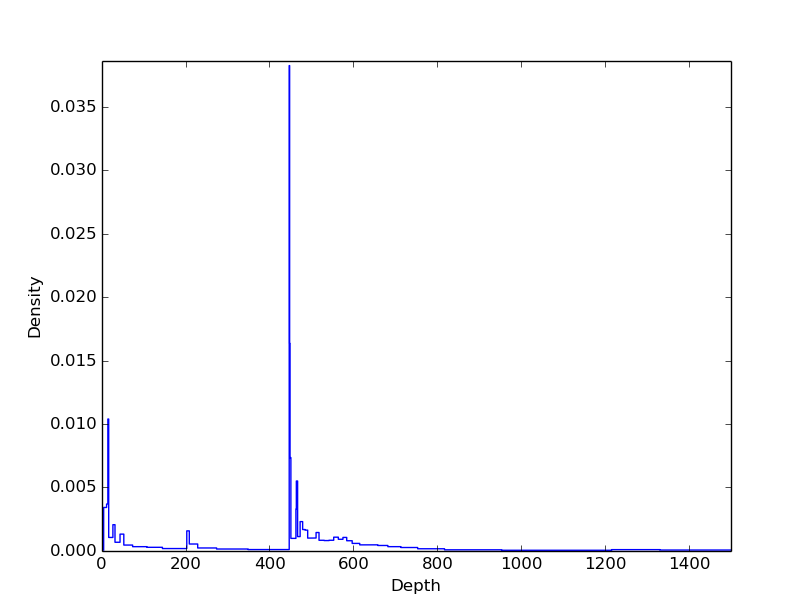
\includegraphics[width=6in]{../media/sdd_financial1_0-1000000.png}
  \caption[SDD of trace Financial1.spc]{This shows the stack depth distribution
  (SDD) for the first 1000000 page requests from Financial1.spc.}
  \label{fig:sdd_financial1}
  \end{figure}

  \begin{figure}
  \centering
  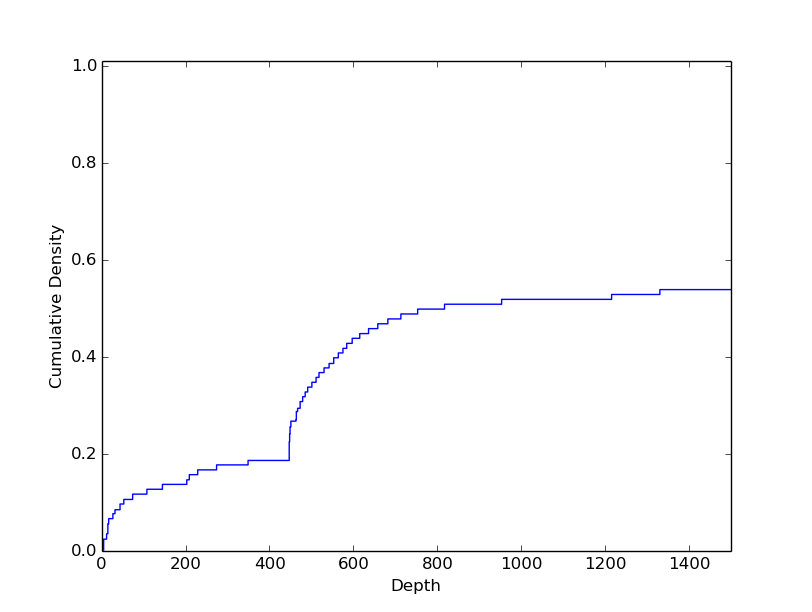
\includegraphics[width=6in]{../media/sdd_cdf_financial1_0-1000000.png}
  \caption[CDF for the SDD of trace Financial1.spc]{This is the cumulative
  distribution function for the stack depth distribution for the first 1000000
  page requests from Financial1.spc. The cumulative value at a depth of 445 is
  12.7\%.}
  \label{fig:sdd_cdf_financial1}
  \end{figure}

  This suggests a few interesting test cases. If we choose a cache size of
  445, the LRU will completely miss the second high density region and the hit
  rate will be limited to $12.7\%$. A good algorithm will be able to identify
  enough important pages that it can cache many of the pages that are only
  referenced again after their depth in the stack depth distribution exceeds
  445. This represents a cache that can only hold 222.5 MB.

  It is worth noting that the bimodality of Figure \ref{fig:sdd_financial1} does
  not indicate that a geometric distribution is a poor model for the stack depth
  distribution. MMC has enough degrees of freedom that it can instead assign
  page requests from the second high density region to the independent reference
  model.

  In order compare how well MMC performs, I created several time-series graphs,
  shown in Figures \ref{fig:ts_445_financial1}, \ref{fig:ts_600_financial1},
  \ref{fig:ts_1000_financial1}, \ref{fig:ts_445_financial2},
  \ref{fig:ts_600_financial2}, and
  \ref{fig:ts_1000_financial2} that chart the cumulative average
  and the rolling average for MMC, LRU, ARC, and MIN.

  \begin{figure}
  \centering
  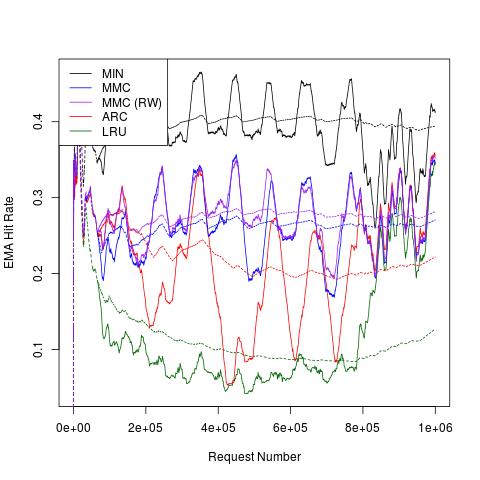
\includegraphics[width=6in]{../media/ts_445_445_1780_2.png}
  \caption[Rolling hit rate for 445 page caches on trace Financial1.spc]{This
  shows the average hit rates (dotted lines) and exponential moving average hit
  rates (solid lines) for several algorithms on the first 1000000 page requests
  in Financial1.spc. The cache size is 445, which is specifically picked because
  the SDD has a high density region starting at a depth of 446. This causes the
  LRU to evict a large number of pages just before they will be requested again.
  The ARC algorithm uses a heuristic that causes it to act like an LRU for large
  portions of this trace. The LRU would have needed to be 11\% longer to achieve
  the same hit rate as ARC and 31\% longer to achieve the same hit rate as
  MMC(RW), which includes the distinction of whether the last reference to a
  page was a read or a write.}
  \label{fig:ts_445_financial1}
  \end{figure}

  \begin{figure}
  \centering
  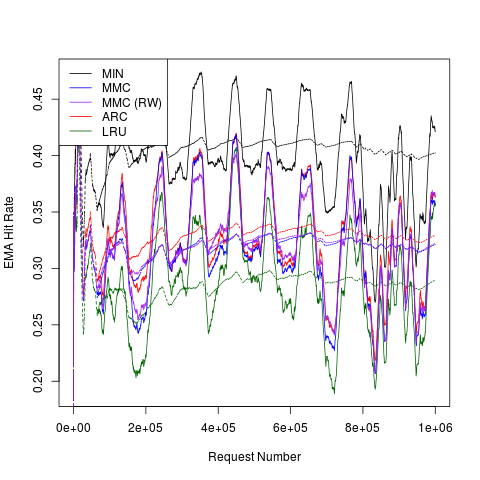
\includegraphics[width=6in]{../media/ts_600_600_2400_2.png}
  \caption[Rolling hit rate for 600 page caches on trace Financial1.spc]{This
  shows the average hit rates (dotted lines) and exponential moving average hit
  rates (solid lines) for several algorithms on the first 1000000 page requests
  in Financial1.spc. The cache size is 600. In certain areas, the hit rates for
  all of the compared algorithms plummets. In these areas, the trace is
  exhibiting the type of behavior expected from a file scan. While the ARC
  algorithm has the best performance on this trace, the MMC algorithms do well
  in the periods just after a file scan. The size of the cache would need to
  have been increased by 26\% for the LRU to achieve the same hit rate as ARC
  and 19\% to match MMC(RW).}
  \label{fig:ts_600_financial1}
  \end{figure}

  \begin{figure}
  \centering
  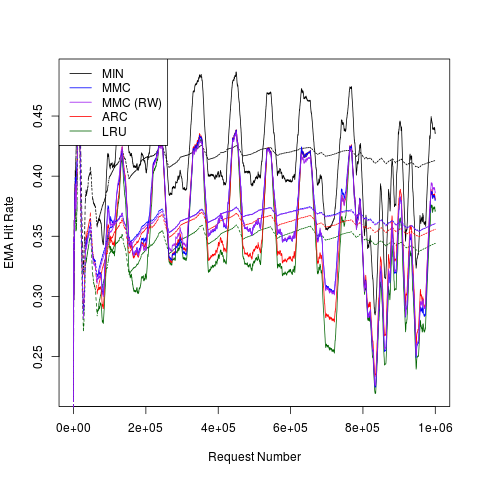
\includegraphics[width=6in]{../media/ts_1000_1000_4000_2.png}
  \caption[Rolling hit rate for 1000 page caches on trace Financial1.spc]{This
  shows the average hit rates (dotted lines) and exponential moving average hit
  rates (solid lines) for several algorithms on the first 1000000 page requests
  in Financial1.spc. The cache size is 1000.}
  \label{fig:ts_1000_financial1}
  \end{figure}

  \begin{figure}
  \centering
  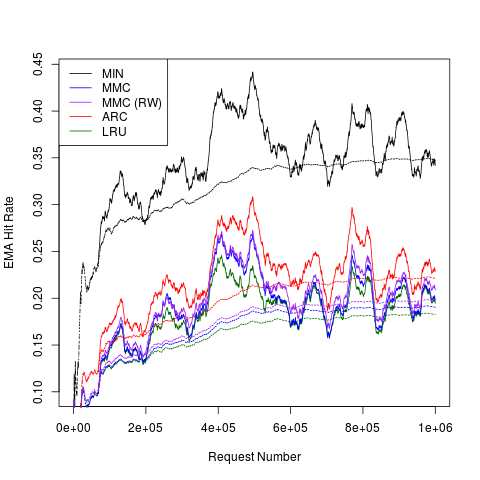
\includegraphics[width=6in]{../media/ts_445_445_1780_3.png}
  \caption[Rolling hit rate for 445 page caches on trace Financial2.spc]{This
  shows the average hit rates (dotted lines) and exponential moving average hit
  rates (solid lines) for several algorithms on the first 1000000 page requests
  in Financial2.spc. The cache size is 445. The LRU cache would need to be 14\%
  larger to have the same hit rate as MMC, 27\% larger to match the hit rate of
  MMC with read/write information, and 83\% larger to match ARC.}
  \label{fig:ts_445_financial2}
  \end{figure}

  \begin{figure}
  \centering
  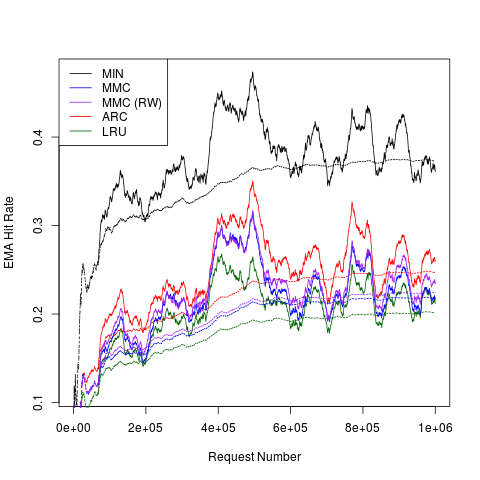
\includegraphics[width=6in]{../media/ts_600_600_2400_3.png}
  \caption[Rolling hit rate for 600 page caches on trace Financial2.spc]{This
  shows the average hit rates (dotted lines) and exponential moving average hit
  rates (solid lines) for several algorithms on the first 1000000 page requests
  in Financial2.spc. The cache size is 600. The hit rate for MMC is equivalent
  to a 28\% larger LRU. MMC with read/write information has the same hit rate as
  a 41\% larger LRU. ARC has the same hit rate as a 90\% larger LRU.}
  \label{fig:ts_600_financial2}
  \end{figure}

  \begin{figure}
  \centering
  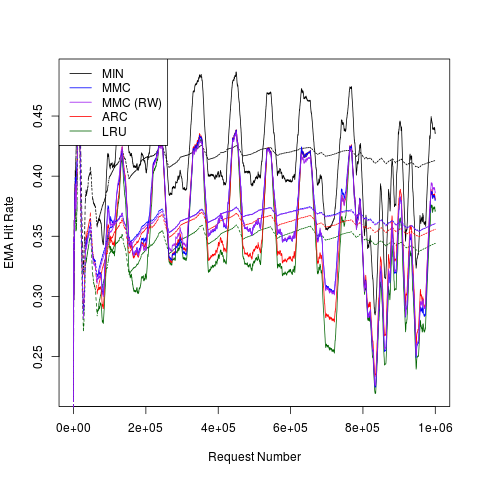
\includegraphics[width=6in]{../media/ts_1000_1000_4000_2.png}
  \caption[Rolling hit rate for 1000 page caches on trace Financial2.spc]{This
  shows the average hit rates (dotted lines) and exponential moving average hit
  rates (solid lines) for several algorithms on the first 1000000 page requests
  in Financial2.spc. The cache size is 1000. A 54\% larger LRU would have the
  same hit rate as MMC, while a 90\% larger LRU would be required to achieve the
  same hit rate as ARC.}
  \label{fig:ts_1000_financial2}
  \end{figure}

  I also compared the performance of MMC on the trace Financial2.spc. The SDD
  for the first 10000000 page requests are shown in Figure
  \ref{fig:sdd_financial2} while the CDF for the SDD is shown in Figure
  \ref{fig:sdd_cdf_financial2}. In sharp contrast to the SDD for Financial1.spc
  shown in Figure \ref{fig:sdd_financial1}, this trace shows a monotonic decay
  that is very suggestive of the geometric distribution. It turns out that the
  MMC algorithm agrees with this assessment the majority of the time, as shown
  by the graph of $\tau_1$ in Figure \ref{fig:tau_and_theta_600_financial2}.

  \begin{figure}
  \centering
  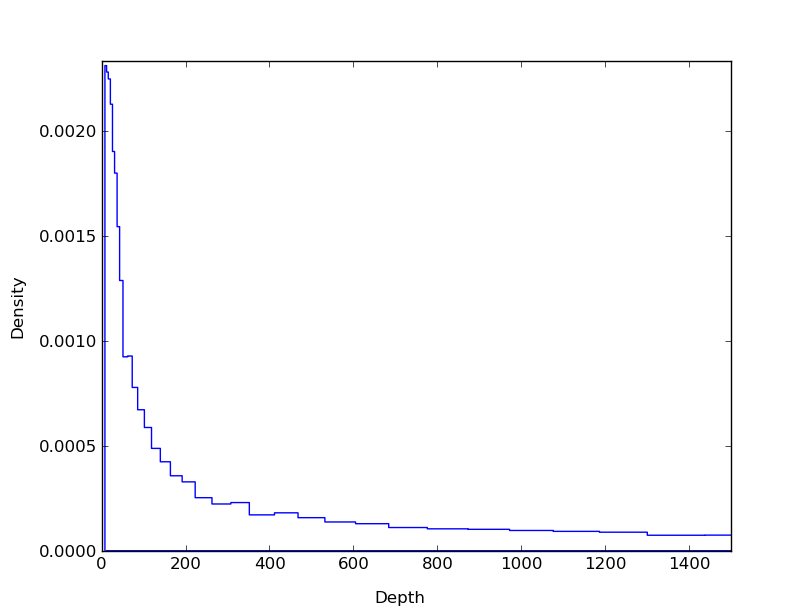
\includegraphics[width=6in]{../media/sdd_financial2_0-1000000.png}
  \caption[SDD of trace Financial2.spc]{This shows the stack depth
  distribution (SDD) for the first 1000000 page requests from Financial1.spc.}
  \label{fig:sdd_financial2}
  \end{figure}

  \begin{figure}
  \centering
  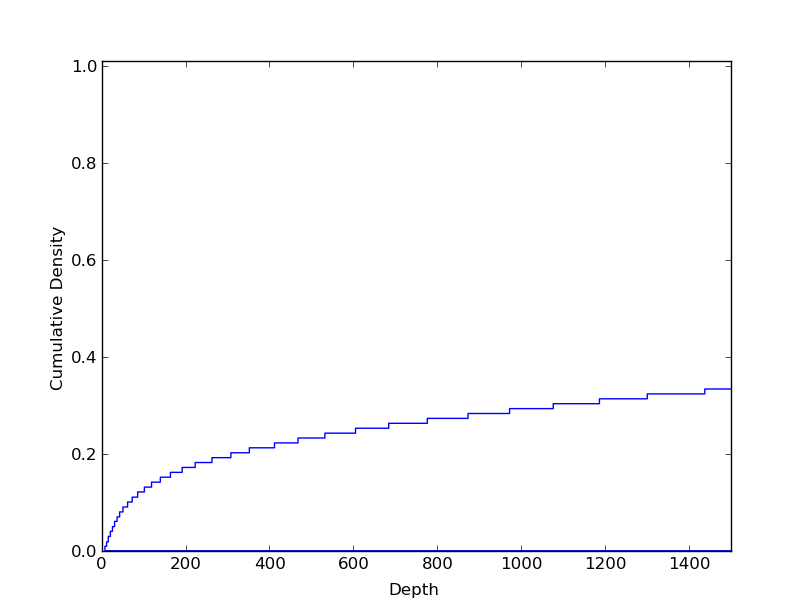
\includegraphics[width=6in]{../media/sdd_cdf_financial2_0-1000000.png}
  \caption[CDF for the SDD of trace Financial2.spc]{This is the cumulative
  distribution function for the stack depth distribution for the first 1000000
  page requests from Financial1.spc. The cumulative value at a depth of 445 is
  12.7\%.}
  \label{fig:sdd_cdf_financial2}
  \end{figure}

  MMC records the relative depth and rank for all pages in cache. Figure
  \ref{fig:ev_1000_financial1} plots these eviction points for all evictions made
  by the two-source MMC algorithm for the first million requests of
  Financial1.spc with a cache that can hold 1000 pages. A few interesting
  features stand out. First, a horizontal line exists at the depth 1000.
  At various points, the value $\tau_1$ is set to the value 1, which is shown in
  Figure \ref{fig:tau_and_theta_1000_financial1}. When $\tau_1 = 1$, the
  algorithm behaves like an LRU. The eviction plot in Figure
  \ref{fig:ev_1000_financial1} also shows two dense eviction regions. These
  correspond to the pages that the algorithm has identified as coming either from
  the independent reference model (this is the region in the top left of the
  graph where the depth of the pages is well over the size of the cache) or from
  the stack depth distribution.

  A small diagonal region at the top right of the graph shows the effect of the
  rolling trace history. When a page is identified as being very important for
  the independent reference model, the algorithm will keep hold of it as long
  as possible. However, the rank of these pages will quickly deteriorate when
  the cluster of references is rolled off the trace.

  A hyperbolically shaped curve exists in Figure \ref{fig:ev_1000_financial1}
  that corresponds to points that could not be cleanly identified as coming from
  the SSD or the IRM. The shape of this curve depends on all of the model
  parameters, but it shows the general relationship that as a page becomes more
  used (i.e., it is highly ranked in the IRM), the algorithm is willing to hold
  onto the page for longer periods of time.

  This graph also shows hints that the mixture model does not have enough
  degrees of freedom to fully capture the memory usage patterns. The most
  obvious issue is the vertical line at rank 1000. If $\tau_2$ were set to 1,
  then MMC would evict pages when their rank exceeds the size of the cache.
  However, as can be seen in Figure \ref{fig:tau_and_theta_1000_financial1},
  $\tau_2$ never equaled 1. Instead, near the end of the trace, the model set
  the value of $\theta_1$ to a very small value that caused the most recent
  pages to be valued so highly that the majority of the distribution was
  essentially flat with an expected value of nearly 0. Since the distribution
  was so flat, the SDD provided very little differentiation between the majority
  of pages. When the value $\theta_1$ was small and $\tau_1$ was not equal to
  1, the relative expected value for pages was determined primarily by
  the IRM.

  \begin{figure}
  \centering
  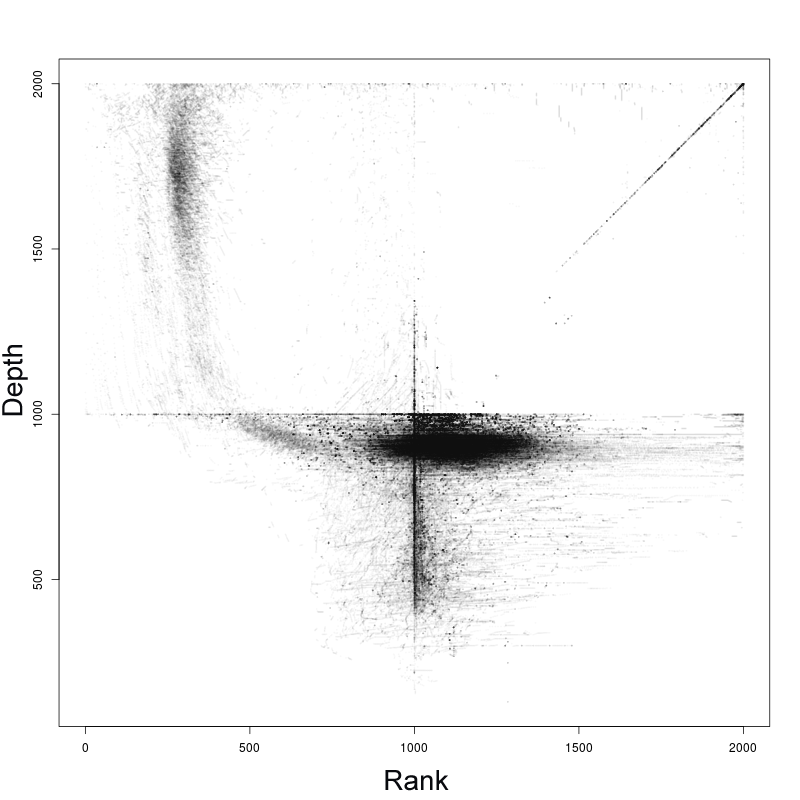
\includegraphics[width=6in]{../media/ev_1000_1000_4000_2.png}
  \caption[Eviction scatterplot for 1000 page MMC cache]{This shows the depth of
  pages in the stack depth distribution (SDD) and the rank of pages in the
  independent reference model (IRM) when they are evicted from the cache by the
  MMC algorithm. The cache can hold 600 pages and can store the metadata for
  another 600 pages. The points in the top right corner represent pages that had
  high rank in the IRM before all of their references rolled off the trace.
  The horizontal line at depth 600 comes from the points in the trace where
  $\tau_1$ equals 1, which causes the algorithm to act like an LRU. The dense
  region in the bottom half of the graph is caused by pages that are assumed to
  be drawn from the SDD. It is denser than the region in the top left of the
  graph because more pages were marked as having come from the SDD than from the
  IRM.}
  \label{fig:ev_1000_financial1}
  \end{figure}

  \begin{figure}
  \centering
  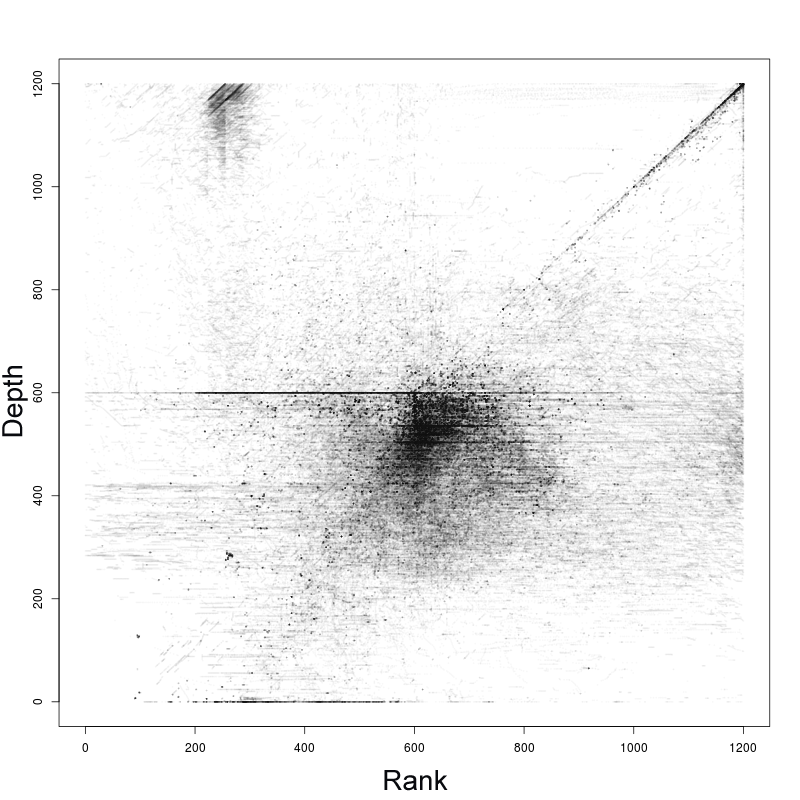
\includegraphics[width=6in]{../media/ev_rw_600_600_2400_2.png}
  \caption[Eviction scatterplot for 1000 page MMC(RW) cache]{This shows the
  depth of pages in the stack depth distribution (SDD) and the rank of pages in
  the independent reference (IRM) model when they are evicted from the cache by
  the MMC(RW) algorithm. The cache can hold 600 pages and can store the
  metadata for another 600 pages. One of the more interesting things about this
  plot is that the algorithm evicted pages with a depth of 0, which means that
  immediately after the pages were requested they were thrown away. When the
  algorithm does not see a request for pages that were recently read or written,
  it decides that the SDD for reads or the SDD for writes is not part of the
  model. Therefore, it assigns a very small expected value to those pages.}
  \label{fig:ev_rw_600_financial1}
  \end{figure}

  \begin{figure}
  \centering
  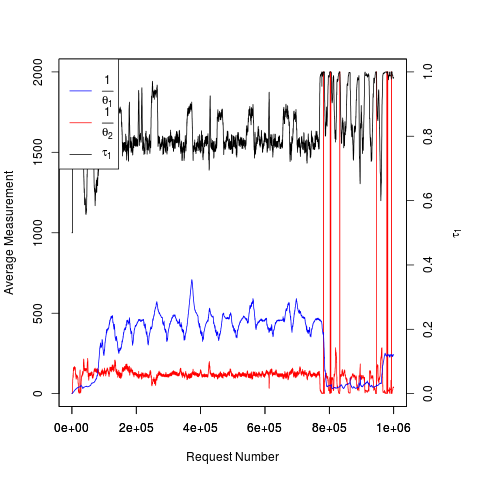
\includegraphics[width=6in]{../media/tau_and_theta_1000_1000_4000_2.png}
  \caption[$\tau_1$, $\frac{1}{\theta_1}$, and $\frac{1}{\theta_2}$ for 1000
  page MMC cache on trace Financial1.spc]
  {This shows all of the model parameters for the two-source MMC
  algorithm with 1000 pages over the first 1000000 page requests on the trace
  Financial1.spc. The value $\tau_1$ ranges between 0 and 1, while the values
  $\frac{1}{\theta_1}$ and $\frac{1}{\theta_2}$ use a scale that shows the
  average value for a page request $X$ drawn from either the SDD modeled with
  $\Geom(H_1(x)|\theta_1)$ or the IRM modeled with $\Geom(H_2(x)|\theta_2)$,
  where the function $H_1$ identifies the depth of page $x$ in the SDD and $H_2$
  identifies the rank of page $x$ in the IRM.}
  \label{fig:tau_and_theta_1000_financial1}
  \end{figure}

  \begin{figure}
  \centering
  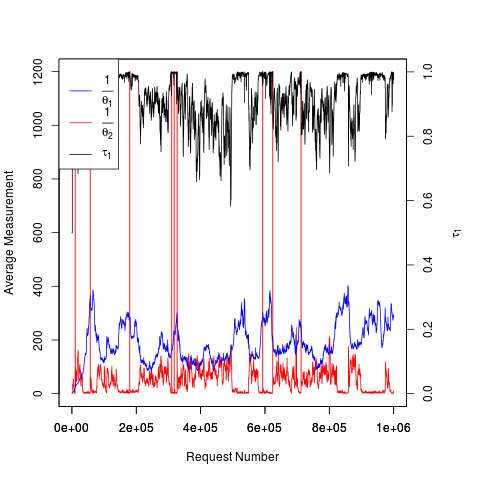
\includegraphics[width=6in]{../media/tau_and_theta_600_600_2400_3.png}
  \caption[$\tau_1$, $\frac{1}{\theta_1}$, and $\frac{1}{\theta_2}$ for 600
  page MMC cache on trace Financial2.spc]{This shows $\tau_1$ for the two-source MMC
  algorithm with 600 pages over the first 1000000 page requests on the trace
  Financial2.spc. When the value of $\tau_1$ is close to 1, MMC behaves much
  like an LRU.}
  \label{fig:tau_and_theta_600_financial2}
  \end{figure}

  We can obtain some insight into how the MMC algorithm works by graphing the
  internal representation of all stored pages. Figure
  \ref{fig:cache_dump_445_financial1} shows a snapshot of the internal
  representation of the pages in the cache. A frozen image doesn't capture the
  dynamic nature of the caching algorithm. The location of pages can change
  drastically after the EM algorithm updates the $\hat{\bm{Z}}$ values for all
  pages. A video showing the internal representation of the pages over time is
  available in the supplemental material \cite{supplimental}.

  \begin{figure}
  \centering
  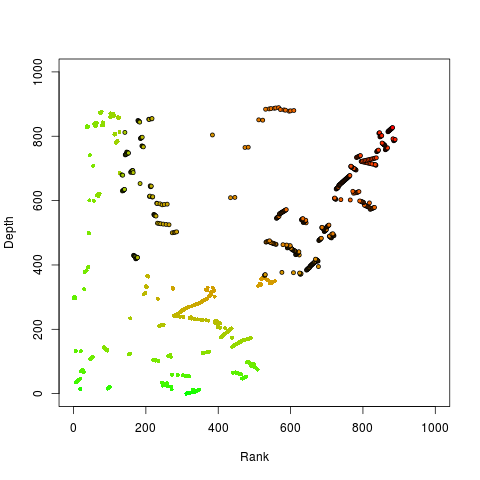
\includegraphics[width=6in]{../media/cache_dump_image_445_445_1780_4_0008090.png}
  \caption[An internal view of a 445 page MMC cache]{This shows a snapshot of
  all pages tracked by the two-source MMC algorithm with 445 pages. Points with
  black circles are evicted pages for which MMC is still storing metadata.}
  \label{fig:cache_dump_445_financial1}
  \end{figure}


\pagebreak

\chapter{Conclusions}
\label{chapter:conclusions}

In this thesis, I have presented a statistical model for a caching algorithm. This
model is unique among caching algorithms because of the flexibility of the
approach, which I demonstrated by extending the algorithm to account for
read/write information. This statistical approach represents a new paradigm in
caching algorithms.

A well-known issue with machine-learning techniques is the variance-bias
tradeoff \cite{intro_to_statistical_learning}. This concept relates to the fact
that the average squared error of a prediction can be decomposed into the
squared bias, which is the consistent and systemic error; the squared variance,
which is the error that occurs because a model is not flexible enough; and an
irreducible error that occurs because some things are just random. A model that
has too few degrees of freedom typically has a large bias, while a model with
too many degrees of freedom will typically has a large variance.

Some caching algorithms, such as the LRU, have no degrees of freedom, which
means that they are unable to adapt to match the data \cite{aho1971principles}.
The ARC algorithm is given a single degree of freedom \cite{arc}. In contrast
with these algorithms, the MMC algorithm is able to incorporate any number of
degrees of freedom.

Furthermore, the MMC algorithm is able to incorporate measurements that cannot
be handled by previous algorithms. I have demonstrated this by deriving a method
that accounts for read/write information. While this model shows promising
results, it also displays some odd behavior. More specifically, the algorithm is
willing to evict the newest pages. While this decision was dictated by the
statistical model, it is contrary behavior to what many people expect from a
caching algorithm.

Even though I supplied a reference implementation, the algorithm is not yet
mature enough to be implemented in a production setting \cite{supplimental}.
The most glaring issue is the execution speed. Most of the phases of the
algorithm take $O(log(|K|))$ time, where $|K|$ is the size of the cache.
However, one portion of the algorithm takes $O(|K|)$ time. This is the phase
where the algorithm recomputes the expected value for all pages in cache.
Several techniques could be employed to reduce this time. Some of these
techniques are outlined in the future work section \ref{chapter:future_work}.

The primary benefits of the MMC algorithm are, first, that it provides a way to
obtain statistical insight into how a process generates page requests, and
second, that it provides a way to use data other than age or frequency when
making caching decisions.


\pagebreak

\chapter{Future Work}
\label{chapter:future_work}

  Several issues need to be resolved before MMC is ready to be tested in a
  production setting. Furthermore, deeper research into particular aspects of
  the MMC algorithm could yield improved performance. In this chapter I outline
  many of these important questions.

\begin{enumerate}

\item
  Can we identify the page with the smallest expected value, or close to the
  smallest expected value, in less than $O(|K|)$ time?

\item
  Can a mixture model be used to provide a caching algorithm that is local to a
  process or a thread, but where the amount of main memory that a process can
  utilize is governed by a mixing parameter?

\item
  If we can estimate the expected headway between faults, can we use this
  information to inform the scheduler?

\item
  Is there any benefit to looking at the relationship between page locations? For
  example, a page hit occurs when the page is re-referenced while it is in
  cache. However, what if we count a reference to page $x + 1$ as a partial
  hit to page $x$?

\item
  Can we use more flexible distribution families to describe the shape of the
  source distributions?

\item
  What other measurements can we take for page requests, and do these
  measurements help improve the hit rate of the MMC algorithm?

\item
  Do alternatives to the EM algorithm exist that require drastically less
  processing time?

\item
  Can a probabilistic model for prefetching be described that will fit into the
  MMC mixture model?

\item
  What design modifications need to be made to use fixed-point arithmetic rather
  than floating-point arithmetic for all of the internal calculations?

Addressing these questions will allow us to take full advantage of the strengths
of the MMC algorithm. Virtual memory is one of the fundamental areas of
systems research, but caches have traditionally been a black box. Development
into statistical cache analysis techniques and algorithms could yield vital
insights and enhancements.

\end{enumerate}


\pagebreak

%References
\addcontentsline{toc}{chapter}{References}

%Relabels bibliography title as "References"
\renewcommand\bibname{References}
\bibliography{yhpargoil}

\end{document}


%% Recommended command line for single figures
%\begin{figure}[!t]
%\centering
%\includegraphics[width=4.5in]{filename}
%\caption{caption text}
%\label{fig:labelTitle}
%\end{figure}


%% Recommended command line for subfigures
%% The current example is set for a figure box that contains 2 subfigures
%% For additional subfigures, the command \begin{subfigure}{.5\textwidth}
%% has to be modified
%\begin{figure}
%\centering
%\begin{subfigure}{.5\textwidth}
%  \centering
%  \includegraphics[scale=0.3]{filenameA}
%  \caption{caption text A}
%  \label{fig:labelTitleA}
%\end{subfigure}%
%\begin{subfigure}{.5\textwidth}
%  \centering
%  \includegraphics[scale=0.3]{filenameB}
%  \caption{caption text B}
%  \label{fig:labelTitleB}
%\end{subfigure}
%\caption{main caption text}
%\label{fig:mainLabelTitle}
%\end{figure}

